\documentclass[14pt]{extarticle} % zmienić na 14 przed wyslaniem tj
 
\usepackage[T1]{fontenc}
\usepackage[utf8]{inputenc}

\usepackage[hidelinks]{hyperref}

\usepackage{microtype}

\usepackage{amssymb}
\usepackage{amsmath}
\usepackage{mathtools}
\usepackage{dsfont}

\usepackage{enumitem}

\usepackage{tikz}
\usetikzlibrary{cd, patterns, patterns.meta, decorations.pathmorphing}

\usepackage{geometry}
\geometry{a4paper, total={170mm, 252mm}, top=22mm}

\usepackage[skip=7pt]{parskip}

\usepackage{amsthm}
\usepackage{thmtools}

\declaretheoremstyle[
    headfont=\bfseries\color{green!80!black},
    bodyfont=\normalfont,
    notebraces={: }{},
    notefont=\color{green},
    headformat=\NAME$\;$\NUMBER\NOTE,
    postheadspace=\newline,
    mdframed={
        linewidth=2pt,
        rightline=false, topline=false, bottomline=false,
        linecolor=green, backgroundcolor=yellow!4,
        skipabove=3mm, skipbelow=3mm
    }
]{defbox}

\declaretheoremstyle[
    headfont=\bfseries\color{orange!80!black},
    bodyfont=\normalfont,
    notebraces={: }{},
    notefont=\color{orange},
    headformat=\NAME$\;$\NUMBER\NOTE,
    postheadspace=\newline,
    mdframed={
        linewidth=2pt,
        rightline=false, topline=false, bottomline=false,
        linecolor=orange, backgroundcolor=yellow!4,
        skipabove=3mm, skipbelow=3mm
    }
]{theorembox}

\declaretheoremstyle[
    headfont=\bfseries\color{blue!80!black},
    bodyfont=\normalfont,
    notebraces={: }{},
    notefont=\color{purple},
    headformat=\NAME$\;$\NUMBER\NOTE,
    postheadspace=\newline,
    mdframed={
        linewidth=2pt,
        rightline=false, topline=false, bottomline=false,
        linecolor=purple, backgroundcolor=yellow!4,
        skipabove=3mm, skipbelow=3mm
    }
]{lemmabox}

\declaretheoremstyle[
    headfont=\bfseries\color{orange!80!black},
    bodyfont=\normalfont,
    notebraces={: }{},
    notefont=\color{orange},
    headformat=\NAME$\;$\NUMBER\NOTE,
    postheadspace=\newline,
    mdframed={
        linewidth=2pt,
        rightline=false, topline=false, bottomline=false,
        linecolor=red!50!orange, backgroundcolor=yellow!4,
        skipabove=3mm, skipbelow=3mm
    }
]{conclusionbox}

\newtheoremstyle{straightstyle}
  {6pt} % Space above
  {6pt} % Space below
  {} % Body font
  {} % Indent amount
  {\bfseries} % Theorem head font
  {.} % Punctuation after theorem head
  {.5em} % Space after theorem head
  {} % Theorem head spec (can be left empty, meaning `normal')

\newtheoremstyle{italicsstyle}
  {6pt} % Space above
  {6pt} % Space below
  {\slshape} % Body font
  {} % Indent amount
  {\bfseries} % Theorem head font
  {.} % Punctuation after theorem head
  {.5em} % Space after theorem head
  {} % Theorem head spec (can be left empty, meaning `normal')

\declaretheorem[ %
  name=Definition, %
  numberwithin=section, %
  style=defbox
]{definition}

\declaretheorem[ %
  name=Theorem, %
  numberwithin=section, %
  style=theorembox
]{theorem}

\declaretheorem[ %
  name=Proposition, %
  numberlike=theorem, %
  style=theorembox
]{proposition}

\declaretheorem[ %
  name=Corollary, %
  numberlike=theorem, %
  style=straightstyle
]{corollary}

\declaretheorem[ %
  name=Lemma, %
  numberlike=theorem, %
  style=lemmabox
]{lemma}

\declaretheorem[ %
  name=Remark, %
  numberlike=definition, %
  style=italicsstyle
]{remark}



\declaretheorem[ %
  name=Conclusion, %
  numberlike=theorem, %
  style=conclusionbox
]{conclusion}

\declaretheorem[ %
  name=Example, %
  numberwithin=section, %
  style=straightstyle
]{example}



% \renewenvironment{proof}{{\bfseries Proof}$ $\newline}{
%   \begin{flushright} $ \spadesuit $ \end{flushright}$ $\newline
% }

\usepackage{cleveref}

%\crefname{definition}{definicja}{definicje}
%\Crefname{definition}{Definicja}{Definicje}
%
%\crefname{theorem}{twierdzenie}{twierdzenia}
%\Crefname{theorem}{Twierdzenie}{Twierdzenia}
%
%\crefname{lemma}{lemat}{lematy}
%\Crefname{lemma}{Lemat}{Lematy}
%
%\crefname{remark}{uwaga}{uwagi}
%\Crefname{remark}{Uwaga}{Uwagi}


\DeclareMathOperator{\Z}{\mathbb{Z}}
\DeclareMathOperator{\R}{\mathbb{R}}
\DeclareMathOperator{\C}{\mathbb{C}}
\DeclareMathOperator{\N}{\mathbb{N}}
\DeclareMathOperator{\Q}{\mathbb{Q}}

\DeclareMathOperator{\im}{im}
\DeclareMathOperator{\coker}{coker}

\newcommand{\set}[1]{\mathcal{#1}}


\DeclareMathOperator{\ord}{ord}
\DeclareMathOperator{\Ann}{Ann}
\DeclareMathOperator{\Hom}{Hom}

\DeclareMathOperator{\End}{End}

\let\landtemp\land
\renewcommand{\land}{\;\landtemp\;}





\usepackage{tikz}
\usetikzlibrary{spath3, hobby, knots, braids}

\pgfdeclarelayer{bg}    % declare background layer
\pgfsetlayers{bg,main}

% Fox colorings and Alexander invariants
\title{ {\bfseries Fox knot colorings and Alexander invariants.}\\ \medskip {\normalsize(Kolorowania Foxa i niezmienniki Alexandera)}}
\author{
  Weronika Jakimowicz\\
  330006
  \and 
  Julia Walczuk\\
  332742
}
\date{\medskip Praca licencjacka 2023-2024}

% \definecolor{red}{HTML}{000000}
% \definecolor{blue}{HTML}{000000}
% \definecolor{orange}{HTML}{000000}
% \definecolor{green}{HTML}{000000}

\begin{document}
\maketitle
\bigskip

\begin{center}
  \large
  \textbf{Promotor:} Lech Tadeusz Januszkiewicz
\end{center}
\vspace{30pt}

\begin{center}
  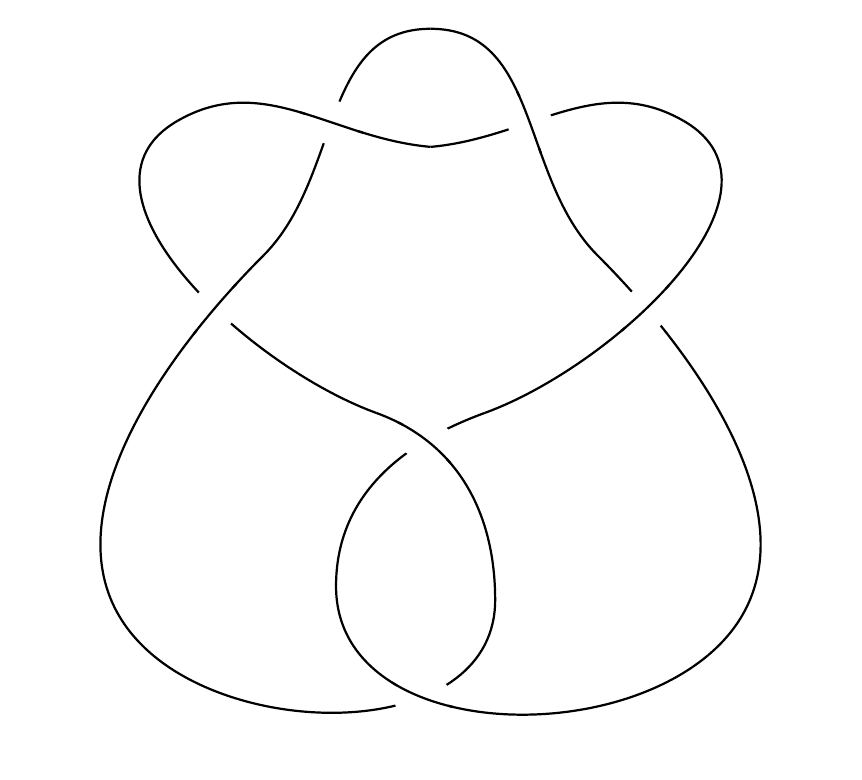
\begin{tikzpicture}[bgnd/.style={circle, fill=white, draw=white}]
    %\node[opacity=0.2] at (0,0) {\includegraphics[width=0.7\textwidth]{./rozdzialy/6_1-3d.png}};

    \coordinate (a0) at (0,0);
    \coordinate (a1) at (90:5);
    \coordinate (a2) at (45:3);
    \coordinate (a3) at (-40:4.6);
    \coordinate (a4) at (-120:2.4);
    \coordinate (a5) at (10:0.7);
    \coordinate (a6) at (50:5);
    \coordinate (a7) at (90:3.5);
    \coordinate (a8) at (180-50:5);
    \coordinate (a9) at (170:0.7);
    \coordinate (a10) at (-70:2.4);
    \coordinate (a11) at (220:4.6);
    \coordinate (a12) at (180-45:3);

    %\foreach \i in {0,...,12} \fill (a\i) circle (2pt);

    \begin{knot}[
      clip width=20,
      flip crossing=1,
      flip crossing=3,
      flip crossing=6
      ]
      \strand[thick] (a1) to[out=0, in=90+45] (a2) to[out=-45, in=40] (a3);
      \strand[thick] (a3) to[out=220, in=-90] (a4) to[out=90, in=200] (a5);
      \strand[thick] (a5) to[out=20, in=-30] (a6);
      \strand[thick] (a6) to[out=150, in=5] (a7);
      \strand[thick] (a7) to[out=175, in=30] (a8);
      \strand[thick] (a8) to[out=210, in=160] (a9);
      \strand[thick] (a9) to[out=-20, in=90] (a10);
      \strand[thick] (a10) to[out=-90, in=-40] (a11);
      \strand[thick] (a11) to[out=140, in=180+45] (a12);
      \strand[thick] (a12) to[out=45, in=180] (a1);
    \end{knot}
  \end{tikzpicture}
\end{center}

\newpage

%\section{Seifert}

\tikzset{
  plusnode/.style={circle, draw=green!60, fill=yellow!5, very thick, minimum size=5mm, scale=0.8, font=\color{green!80!red}\bfseries},
  minusnode/.style={circle, draw=blue!60, fill=orange!5, very thick, minimum size=5mm, scale=0.8, font=\color{blue!80!red}\bfseries}
}

Na \cref{pow61} jest powierzchnia Seiferta $6_1$, kolory oznaczają pętelki-generatory.

Moduł Alexandera wychodzi $\Z[\Z]/(-2t^2+5t-2)$, czyli nic niezwykłego.

\begin{figure}[h]\centering
  \begin{tikzpicture}
  \draw (0,0) circle (1);
  \draw (0,0) ellipse (2.5 and 3.5);
  \draw (6, 0) circle (1);
  \draw (4.5, 3) circle (1);
  \draw (4.5, -3) circle (1);
  
  \coordinate (firstEnd) at ({2.5 * cos(8)}, {3.5 * sin(8)});
  \coordinate (secondEnd) at ({2.5 * cos(-8)}, {3.5 * sin(-8)});

  \draw ({cos(30)}, {sin(30)}) to [out=0, in=180] (secondEnd);
  \fill[white] (1.7, 0) circle (4pt);
  \draw ({cos(-30)}, {sin(-30)}) to[out=0, in=180] (firstEnd);
  \draw[ultra thick, white] ({cos(29)}, {sin(29)}) arc (29:-29:1);

  \coordinate (firstEnd) at ({-2.5 * cos(8)}, {3.5 * sin(8)});
  \coordinate (secondEnd) at ({-2.5 * cos(-8)}, {3.5 * sin(-8)});

  \draw ({-cos(-30)}, {sin(-30)}) to[out=180, in=0] (firstEnd);
  \fill[white] (-1.7, 0) circle (4pt);
  \draw ({-cos(30)}, {sin(30)}) to[out=180, in=0] (secondEnd);
  \draw[ultra thick, white] ({-cos(29)}, {sin(29)}) arc (180-29:180+29:1);

  \coordinate (a1) at ({2.5 * cos(45)}, {3.5 * sin(45)});
  \coordinate (a2) at ({2.5 * cos(70)}, {3.5 * sin(70)});
  
  \draw[ultra thick, white] (a1) arc (45:70:2.5 and 3.5);

  \begin{scope}[shift={(4.5, 3)}] 
    \coordinate (a3) at ({-cos(30)}, {sin(30)});
    \coordinate (a4) at ({-cos(-30)}, {sin(-30)});
    \draw[ultra thick, white] (a3) arc (180-30:180+30:1);
  \end{scope}
  
  \begin{scope}[shift={(4.5, -3)}] 
    \coordinate (a5) at ({-cos(30)}, {sin(30)});
    \coordinate (a6) at ({-cos(-30)}, {sin(-30)});
    \draw[ultra thick, white] (a5) arc (180-30:180+30:1);
  \end{scope}
  
  \coordinate (a7) at ({2.5 * cos(-45)}, {3.5 * sin(-45)});
  \coordinate (a8) at ({2.5 * cos(-70)}, {3.5 * sin(-70)});

  \draw[ultra thick, white] (a7) arc (-45:-70:2.5 and 3.5);

  %\foreach \i in {1,...,8} \fill (a\i) circle (4pt) node [above] {\i};

  \draw[name path=a1-3] (a1) to[out=70, in=180] (a3);
  \draw[white, name path=a2-4] (a2) to[out=45, in=180] (a4);
  \path [name intersections={of=a1-3 and a2-4, by=A1}];
  \fill[white] (A1) circle (4pt);
  \draw (a2) to[out=45, in=180] (a4);
  
  \draw[white, name path=a7-6] (a7) to[out=-45, in=180] (a6);
  \draw[name path=a8-5] (a8) to[out=-70, in=180] (a5);
  \path [name intersections={of=a7-6 and a8-5, by=A2}];
  \fill[white] (A2) circle (4pt);
  \draw (a7) to[out=-45, in=180] (a6);

  \begin{scope}[shift={(6, 0)}]
    \coordinate (b1) at ({cos(90-30)}, {sin(90-30)});
    \coordinate (b2) at ({cos(90+30)}, {sin(90+30)});

    \coordinate (b3) at({cos(-90-30)}, {sin(-90-30)});
    \coordinate (b4) at({cos(-90+30)}, {sin(-90+30)});
  \end{scope}

  \begin{scope}[shift={(4.5, 3)}]
    \coordinate (b5) at ({cos(-90+30)}, {sin(-90+30)});
    \coordinate (b6) at (1, 0);
  \end{scope}

  \begin{scope}[shift={(4.5, -3)}]
    \coordinate (b7) at (1, 0);
    \coordinate (b8) at ({cos(90-30)}, {sin(90-30)});
  \end{scope}
  
  %\foreach \i in {1,...,8} \fill (b\i) circle (4pt) node [above] {\i};
  
  \draw[white, ultra thick] (b6) arc (0:-60:1);
  \draw[white, ultra thick] (b2) arc (120:60:1);
  \draw[ultra thick, white] (b3) arc (-90-30:-90+30:1);
  \draw[ultra thick, white] (b8) arc (60:0:1);

  \draw[name path=b5-1] (b5) to[out=-60, in=90] (b1);
  \draw[name path=b6-2, white] (b6) to[out=0, in=90] (b2);
  \path[name intersections={of=b5-1 and b6-2, by=B1}];
  \fill[white] (B1) circle (4pt);
  \draw (b6) to[out=0, in=90] (b2);

  \draw[name path=b7-3] (b7) to[out=60, in=-90] (b3);
  \draw[name path=b8-4, white] (b8) to[out=0, in=-90] (b4);
  \path[name intersections={of=b7-3 and b8-4, by=B2}];
  \fill[white] (B2) circle (4pt);
  \draw (b8) to[out=0, in=-90] (b4);

  \draw[thick, purple, ->] (4.5, 3) to[out=180, in=0] 
    (A1) to[out=180, in=90] 
    (1.5, 2);
  \draw[thick, purple, ->] (1.5, 2) to[out=-90, in=90]
    (1.5, -2);
  \draw[thick, purple, ->] (1.5, -2) to[out=-90, in=180]
    (A2) to[out=0, in=180]
    (4.5, -3);
  \draw[thick, purple, ->] (4.5, -3) to[out=0, in=240]
    (B2) to[out=60, in=-90] 
    (6, 0);
  \draw[purple, thick, ->] (6, 0) to[out=90, in=-60]
    (B1) to[out=120, in=0]
    (4.5, 3);

  \draw[thick, purple, ->] (0,-0.3) to[out=160, in=-70] (-2.5, 0.6);
  \draw[thick, purple, ->] (-2.5, 0.6) to[out=90, in=180] (0, 1.5);
  \draw[thick, purple, ->] (0, 1.5) to[out=0, in=90] (2.5, 0.6);
  \draw[thick, purple, ->] (2.5, 0.6) to[out=-110, in=20] (0,-0.3);

  \node at (0, -0.7) {$\color{purple}a$};
  \node at (6.4, 0) {$\color{purple}b$};

  \node[plusnode] at (0,0.4) {$+$};
  \node[plusnode] at (5.45, 0) {$+$};
  \node[plusnode] at (-1, 2.3) {$+$};

  \node[minusnode] at (4.2, 3.5) {$-$};
  \node[minusnode] at (4.2, -3.5) {$-$};
\end{tikzpicture}

\caption{\label{pow61}Powierzchnia Seiferta $6_1$.}
\end{figure}


Powierzchnia Seiferta węzła $9_{46}$ jest z kolei na \cref{pow946} i nie wychodzi ładnie. To znaczy, relacje po rozpisaniu wyglądają następująco (nad znakami równości z których czerwonych pętelek przychodzą, pozostałe to obserwacje obrazku):
\begin{align*}
  ta^- &\overset{a}{=} X-f^--a^-\\ 
  0&\overset{b}{=}-Y+E+a^-\\ 
  tX+tC&\overset{c}{=}c^+\\ 
  -tY&\overset{d}{=}c^+ \\ 
  tZ-tE&\overset{e}{=}-Y+G\\ 
  tf^- &\overset{f}{=}Z-c^++X\\ 
  C-G&=c^+\\ 
  0&=X+Y+Z
\end{align*}
\begin{figure}[h]\centering
  \begin{tikzpicture}
  \begin{scope}
    \draw (0,0) circle (1);
    \draw (0,0) ellipse (2.5 and 3.5);
    
    \coordinate (B1) at ({cos(180-20)-1.5}, {sin(180-20)});
    \coordinate (A1) at ({cos(180+20)-1.5}, {sin(180+20)});

    \coordinate (B0) at (360/3-90:2.5 and 3.5);
    \coordinate (A0) at (360/3+20-90:2.5 and 3.5);

    \coordinate (B2) at (2*360/3-30+100:2.5 and 3.5);
    \coordinate (A2) at (2*360/3-10+100:2.5 and 3.5);

    \foreach \i in {0,1,2} {
      \coordinate (a\i) at (\i*360/3 + 60+20:1);
      \coordinate (b\i) at (\i*360/3 + 60-20:1);

      % \fill (a\i) circle (4pt) node [above] {a\i};
      % \fill (b\i) circle (4pt) node [above] {b\i};
      %
      % \fill (A\i) circle (4pt) node [above] {A\i};
      % \fill (B\i) circle (4pt) node [above] {B\i};
    }

    \coordinate (c1) at (90+20:2.5 and 3.5);
    \coordinate (c2) at (90-20:2.5 and 3.5);
    \coordinate (c3) at (15:2.5 and 3.5);
    \coordinate (c4) at (-15:2.5 and 3.5);
    \coordinate (c5) at (-90+20:2.5 and 3.5);
    \coordinate (c6) at (-90-20:2.5 and 3.5);

    % \foreach \i in {1,..., 6} \fill (c\i) circle (4pt) node[above] {c\i};
    \draw[ultra thick,white] (c1) arc (110:70:2.5 and 3.5);
    \draw[ultra thick,white] (c3) arc (15:-15:2.5 and 3.5);
    \draw[ultra thick,white] (c5) arc (-70:-110:2.5 and 3.5);
  \end{scope}

  
  \begin{scope}[shift={(7, 0)}]
    \draw (0,0) circle (1);
    \draw (0,0) ellipse (2.5 and 3.5);

    \coordinate (D0) at ({cos(-20)+1.5}, {sin(-20)});
    \coordinate (E0) at ({cos(20)+1.5}, {sin(20)});
    \coordinate (D1) at (360/3+10:2.5 and 3.5);
    \coordinate (E1) at (360/3+30:2.5 and 3.5);
    \coordinate (D2) at (2*360/3-30:2.5 and 3.5);
    \coordinate (E2) at (2*360/3-10:2.5 and 3.5);

    \foreach \i in {0,1,2} {
      \coordinate (d\i) at (\i*360/3-20:1);
      \coordinate (e\i) at (\i*360/3+20:1);

      % \fill (d\i) circle (4pt) node [above] {d\i};
      % \fill (e\i) circle (4pt) node [above] {e\i};
      %
      % \fill (D\i) circle (4pt) node [above] {D\i};
      % \fill (E\i) circle (4pt) node [above] {E\i};
    }

    \coordinate (f1) at (90-20:2.5 and 3.5);
    \coordinate (f2) at (90+20:2.5 and 3.5);
    \coordinate (f3) at (180-15:2.5 and 3.5);
    \coordinate (f4) at (180+15:2.5 and 3.5);
    \coordinate (f5) at (-90-20:2.5 and 3.5);
    \coordinate (f6) at (-90+20:2.5 and 3.5);
    
    \draw[ultra thick,white] (f2) arc (110:70:2.5 and 3.5);
    \draw[ultra thick,white] (f3) arc (180-15:180+15:2.5 and 3.5);
    \draw[ultra thick,white] (f6) arc (-70:-110:2.5 and 3.5);

    % \foreach \i in {1,..., 6} \fill (f\i) circle (4pt) node[above] {f\i};
  \end{scope}

  \draw[name path=c1-f2, white] (c1) to[out=90, in=90] (f2);
  \draw[name path=c2-f1] (c2) to[out=90, in=90] (f1);
  \path[name intersections={of=c1-f2 and c2-f1, by=CF1}];
  \fill[white] (CF1) circle (15pt);
  \draw (c1) to[out=90, in=90] (f2);

  \draw[name path=c5-f6] (c5) to[out=-90, in=-90] (f6);
  \draw[name path=c6-f5, white] (c6) to[out=-90, in=-90] (f5);
  \path[name intersections={of=c5-f6 and c6-f5, by=CF2}];
  \fill[white] (CF2) circle (15pt);
  \draw (c6) to[out=-90, in=-90] (f5);

  \draw[name path=c3-f4, white] (c3) to[out=0, in=180] (f4);
  \draw[name path=c4-f3] (c4) to[out=0, in=180] (f3);
  \path[name intersections={of=c3-f4 and c4-f3, by=CF3}];
  \fill[white] (CF3) circle (6pt);
  \draw (c3) to[out=0, in=180] (f4);

  \foreach \i in {0,2} {
    \draw[ultra thick, white] (e\i) arc (\i*120+20:\i*120-30:1);

    \draw[name path=u\i, white] (e\i) to[out=360/3*\i, in=180+\i*360/3] (D\i);
    \draw[name path=t\i] (d\i) to[out=360/3*\i, in=180+\i*360/3] (E\i);
    \path[name intersections={of={u\i} and {t\i}, by=DE\i}];
    \fill[white] (DE\i) circle (6pt);
    \draw (e\i) to[out=360/3*\i, in=180+\i*360/3] (D\i);
  }
  \foreach \i in {1} {
    \draw[ultra thick, white] (e\i) arc (\i*120+20:\i*120-30:1);

    \draw[name path=u\i] (e\i) to[out=360/3*\i, in=180+\i*360/3] (D\i);
    \draw[name path=t\i, white] (d\i) to[out=360/3*\i, in=180+\i*360/3] (E\i);
    \path[name intersections={of={u\i} and {t\i}, by=DE\i}];
    \fill[white] (DE\i) circle (6pt);
    \draw (d\i) to[out=360/3*\i, in=180+\i*360/3] (E\i);
  }


  \foreach \i in {1,2} {
    \draw[ultra thick, white] (a\i) arc (\i*120+60+20:\i*120+60+20-30:1);

    \draw[name path=s\i, white] (a\i) to[out=360/3*\i+60, in=\i*360/3-120] (B\i);
    \draw[name path=r\i] (b\i) to[out=360/3*\i+60, in=\i*360/3-120] (A\i);
    \path[name intersections={of={s\i} and {r\i}, by=AB\i}];
    \fill[white] (AB\i) circle (6pt);
    \draw (a\i) to[out=360/3*\i+60, in=\i*360/3-120] (B\i);
  }
  \foreach \i in {0} {
    \draw[ultra thick, white] (a\i) arc (\i*120+60+20:\i*120+60+20-30:1);

    \draw[name path=s\i] (a\i) to[out=360/3*\i+60, in=\i*360/3-120] (B\i);
    \draw[name path=r\i,white] (b\i) to[out=360/3*\i+60, in=\i*360/3-120] (A\i);
    \path[name intersections={of={s\i} and {r\i}, by=AB\i}];
    \fill[white] (AB\i) circle (6pt);
    \draw (b\i) to[out=360/3*\i+60, in=\i*360/3-120] (A\i);
  }

  \draw[thick, purple, ->] (CF1) to[out=180, in=90] (0, 3.5);
  \draw[thick, purple, ->] (0, 3.5) to[out=-90, in=160] (2.7, 0.5);
  \draw[thick, purple, ->] (2.7, 0.5) to[out=-20, in=180] (3.5, 0.05) to[out=0, in=200] (4.3, 0.5);
  \draw[thick, purple, ->] (4.3, 0.5) to[out=20, in=-90] (7, 3.5);
  \draw[thick, purple, ->] (7, 3.5) to[out=90, in=0] (CF1);
  \node at (3.7, 5) {$\color{purple}e$};
  
  \draw[thick, purple, ->] (CF2) to[out=180, in=-90] (0, -3.5);
  \draw[thick, purple, ->] (0, -3.5) to[out=90, in=200] (2.7, -0.5);
  \draw[thick, purple, ->] (2.7, -0.5) to[out=20, in=180] (3.5, -0.05) to[out=0, in=160] (4.3, -0.5);
  \draw[thick, purple, ->] (4.3, -0.5) to[out=-20, in=90] (7, -3.5);
  \draw[thick, purple, ->] (7, -3.5) to[out=-90, in=0] (CF2);
  \node at (3.7, -5) {$\color{purple}f$}; 



  \draw[thick, purple, ->] (0,0.5) to[out=210, in=0] ([yshift=2pt]AB1) 
  to[out=180, in=-90] (175:2.5 and 3.5)
  to[out=90, in=210] (-0.8, 1.8);
  \draw[thick, purple, ->] (-0.8, 1.8) to[out=30, in=90] (40:2.5 and 3.5) 
  to[out=-90, in=60] ([yshift=2pt]AB0) to[out=240, in=30] (0, 0.5);
  
  \draw[thick, purple, ->] (0, -0.5) to[out=150, in=0] ([yshift=-2pt]AB1) 
  to[out=180, in=90] (185:2.5 and 3.5)
  to[out=-90, in=150] (-0.8, -1.8);
  \draw[thick, purple, ->] (-0.8, -1.8) to[out=-30, in=-90] (-40:2.5 and 3.5)
  to[out=90, in=-60] ([yshift=-2pt]AB2) to[out=120, in=-30] (0, -0.5);


  \begin{scope}[shift={(7, 0)}]
    \draw[thick, purple, ->] (0,0.5) to[out=150, in=-60] ([yshift=2pt]DE1) 
    to[out=120, in=-90] (180-40:2.5 and 3.5)
    to[out=90, in=150] (0.8, 1.8);
    \draw[thick, purple, ->] (0.8, 1.8) to[out=-30, in=90] (5:2.5 and 3.5) 
    to[out=-90, in=-30] ([yshift=2pt]DE0) to[out=150, in=-30] (0, 0.5);
  
    \draw[thick, purple, ->] (0, -0.5) to[out=210, in=60] ([yshift=-2pt]DE2) 
    to[out=240, in=90] (180+40:2.5 and 3.5)
    to[out=-90, in=210] (0.8, -1.8);
    \draw[thick, purple, ->] (0.8, -1.8) to[out=30, in=-90] (-5:2.5 and 3.5)
    to[out=90, in=-30] ([yshift=-2pt]DE0) to[out=150, in=30] (0, -0.5);
  \end{scope}

  \node at (-0.8, 2.2) {$\color{purple}b$};
  \node at (-0.8, -2.2) {$\color{purple}a$};
  \node at (7.8, 2.2) {$\color{purple}d$};
  \node at (7.8, -2.2) {$\color{purple}c$};

  \draw[->, thick, blue] (2, 5.5) arc (170:-130:0.5 and 1);
  \node at (1.8, 6) {$\color{blue}Y$};

  \draw[->, thick, blue] (3, 0.9) arc (120:-120:0.5 and 1.1);
  \node at (3.1, 1.3) {$\color{blue}Z$};

  \draw[->, thick, blue] (2, -4.7) arc (170:-130:0.5 and 1);
  \node at (1.8, -5.2) {$\color{blue}X$};

  \draw[->, thick, blue] ([xshift=-6pt, yshift=6pt]AB0) arc (170:-110:0.3 and 0.7); 
  \node at ([yshift=-25pt, xshift=10pt]AB0) {$\color{blue}E$};

  \draw[->, thick, blue] ([yshift=10pt]DE1) arc (120:-180:0.3 and 0.7);
  \node at ([yshift=-25pt, xshift=-15pt]DE1) {$\color{blue}G$};

  \draw[->, thick, blue] ([yshift=10pt]DE0) arc (160:-150:0.3 and 0.7);
  \node at ([yshift=-25pt]DE0) {$\color{blue}C$};

  \node[plusnode] at (7,0) {$+$};
  \node[plusnode] at (8, 2.7) {$+$};
  \node[minusnode] at (0, 0) {$-$};
  \node[minusnode] at (-1, 2.7) {$-$};
\end{tikzpicture}

  \caption{\label{pow946}Powierzchnia Seiferta $9_{46}$.}
\end{figure}

Z tych równań wyciągam tylko tyle, że 
$$Z(1-t)+X(1-2t)+a^-(t^2+t)=0$$
oraz
$$Y(3t^2+2t-3)=X(1+t-t^2).$$
Moim zdaniem powinno wyjść coś z dwoma generatorami, ale jeszcze nie wymyśliłam jak je wyciągnąć.

\section{Relacja na macierzach}

% Nie wzięłam ze sobą zeszytu, w którym mazałam we Wrocławiu, więc musiałam ten problem od zera rozpisywać i coś mi się przestało zgadzać. Zaczęłam od przykładów.
Nie mam aktualnie zeszytu w którym pracowałam do tej pory, więc zaczęłam od przykładów.

\begin{center}
  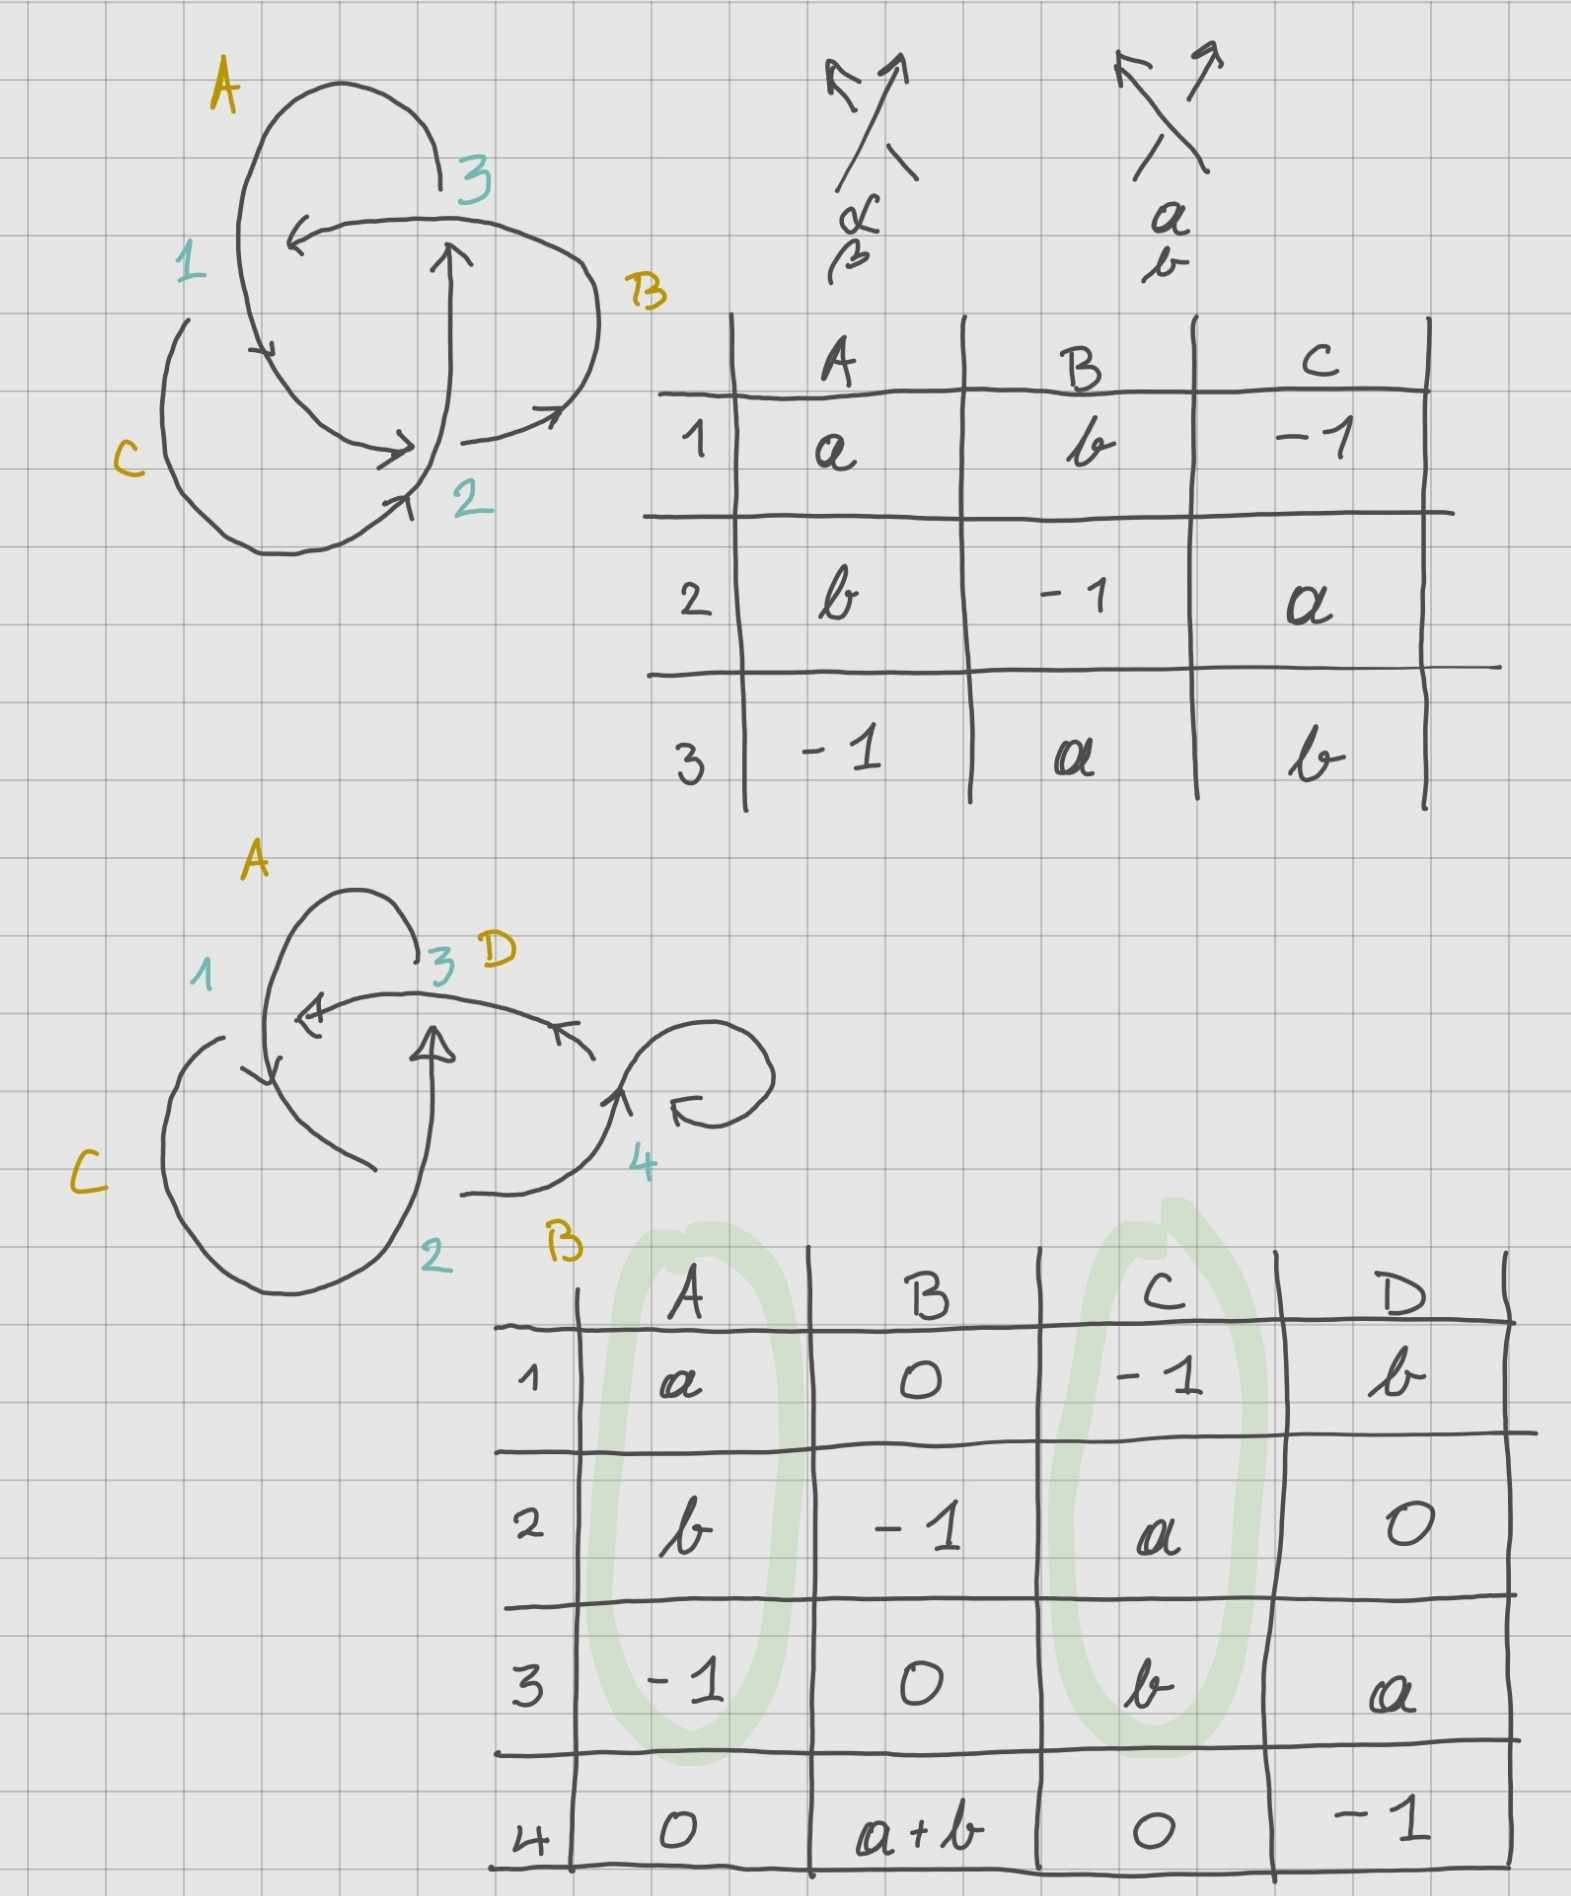
\includegraphics[width=\textwidth]{./rozdzialy/relacja_trefl_1.jpg}
\end{center}
\newpage 

Diagramiki skrzyżowań w prawym górnym rogu oznaczają, które skrzyżowanie ma $au+bi=-o$, a które $\alpha u+\beta i=-o$.

Niech $D$ będzie diagramem po usunięciu kinku, a $D'$ przed (góra-dół na rysunku). Dla prostoty $D:M^s\to N^x$ i $D:M^{s+1}\to N^{x+1}$ to macierze powstałe z odpowiednich diagramów.

Wtedy kolumny łuczków w $D$, które nie plączemy (ich jest $s-1$ sztuk) są bez zmiany, czyli 
$$D(M^{s-1})=D'(M^{s-1}).$$
Dodatkowo, jeśli $M_s$ jest łuczkiem, który zaplątaliśmy (ostatnia współrzędna, na obrazku troszkę nie wyszło), a $M_{s+1}$ łuczkiem, który przez zaplątanie powstał, to chcemy, żeby 
$$(D'(M_s)+ D'(M_{s+1}))\cap N^x=D(M_s),$$
gdzie to przecięcie po lewej stronie rozumiemy jako ograniczenie się do pierwszych $x$ współrzędnych powstałego wektora ($x+1$-sza to nowe skrzyżowanie).

\newpage 

\begin{center}
  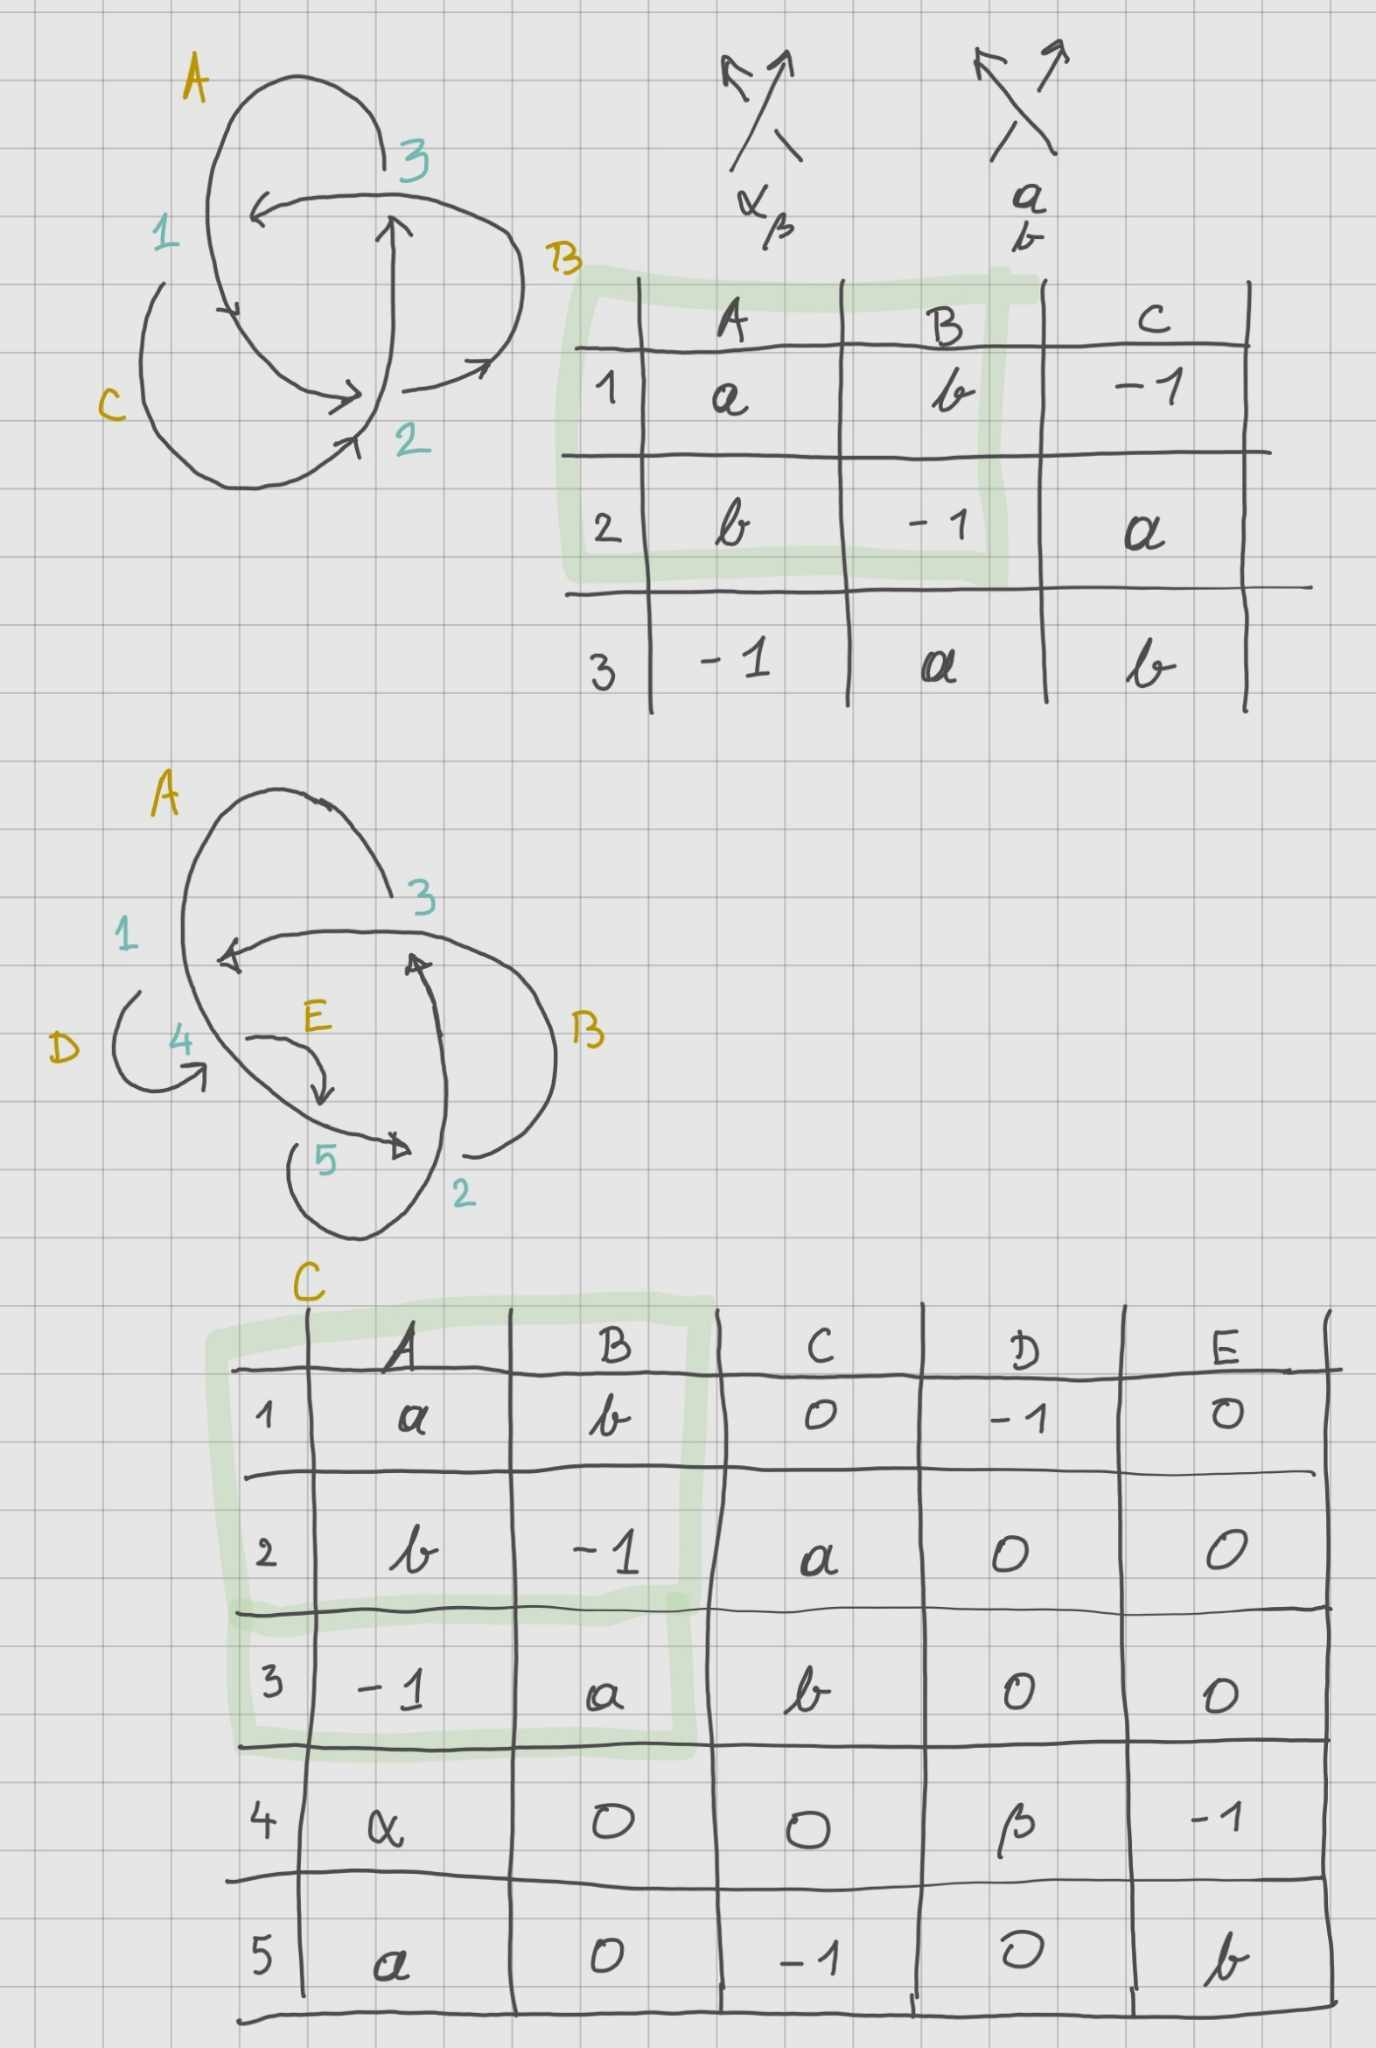
\includegraphics[width=\textwidth]{./rozdzialy/relacja_trefl_2.jpg}
\end{center}
\newpage 

W tym ruchu wyjęcia nitki spod spodu naruszyliśmy tylko jeden łuczek w diagramie po wyjęciu $D$ (diagram przed wyciągnięciem to $D'$). W takim razie, podobnie jak wcześniej chcemy
$$D(M^{s-1})=D'(M^{s-1})\cap N^x.$$
Możemy posunąć się dalej, i jeśli pierwsza nitka $M_1$ to ta, spod której wyjmowaliśmy, to chcemy 
$$(D(M^{s-1}), 0, 0)=D'(M^{s-1})-\omega_+(M_1, 0, 0)-\omega_-(M_1, 0, 0),$$
gdzie $\omega_\pm(u, i, o)$ to funkcja kolorująca odpowiadająca za każdy z rodzai skrzyżowań, jaki powstał przez wsunięcie pod $M_1$ nitki $M_s$. Oczywiście, musimy wiedzieć, które skrzyżowanie w $D'$ to który rodzaj skrzyżowania i umieścić $\omega_\pm(M_1,0,0)$ na odpowiedniej współrzędnej. 

Ta część wydaje mi się nieco brzydka. Po prostu chciałam jakoś zaakcentować fakt, że na ostatnich dwóch wierszach jedna nitka ma zawsze być górą i ma być górą na dwa różne sposoby.

Pozostaje powiedzieć, że fragmenty wsuniętej nitki dodają się do tego, co widzimy w nitce przed byciem wsuwaną:
$$D(M_s)=[D'(M_s)+D'(M_{s+1})+D'(M_{s+2})]\cap N^x$$

Pozostaje ostatni ruch Reidenmeistera oraz (chyba) napisanie tego samego dla odwrotnej orientacji.

\begin{center}
  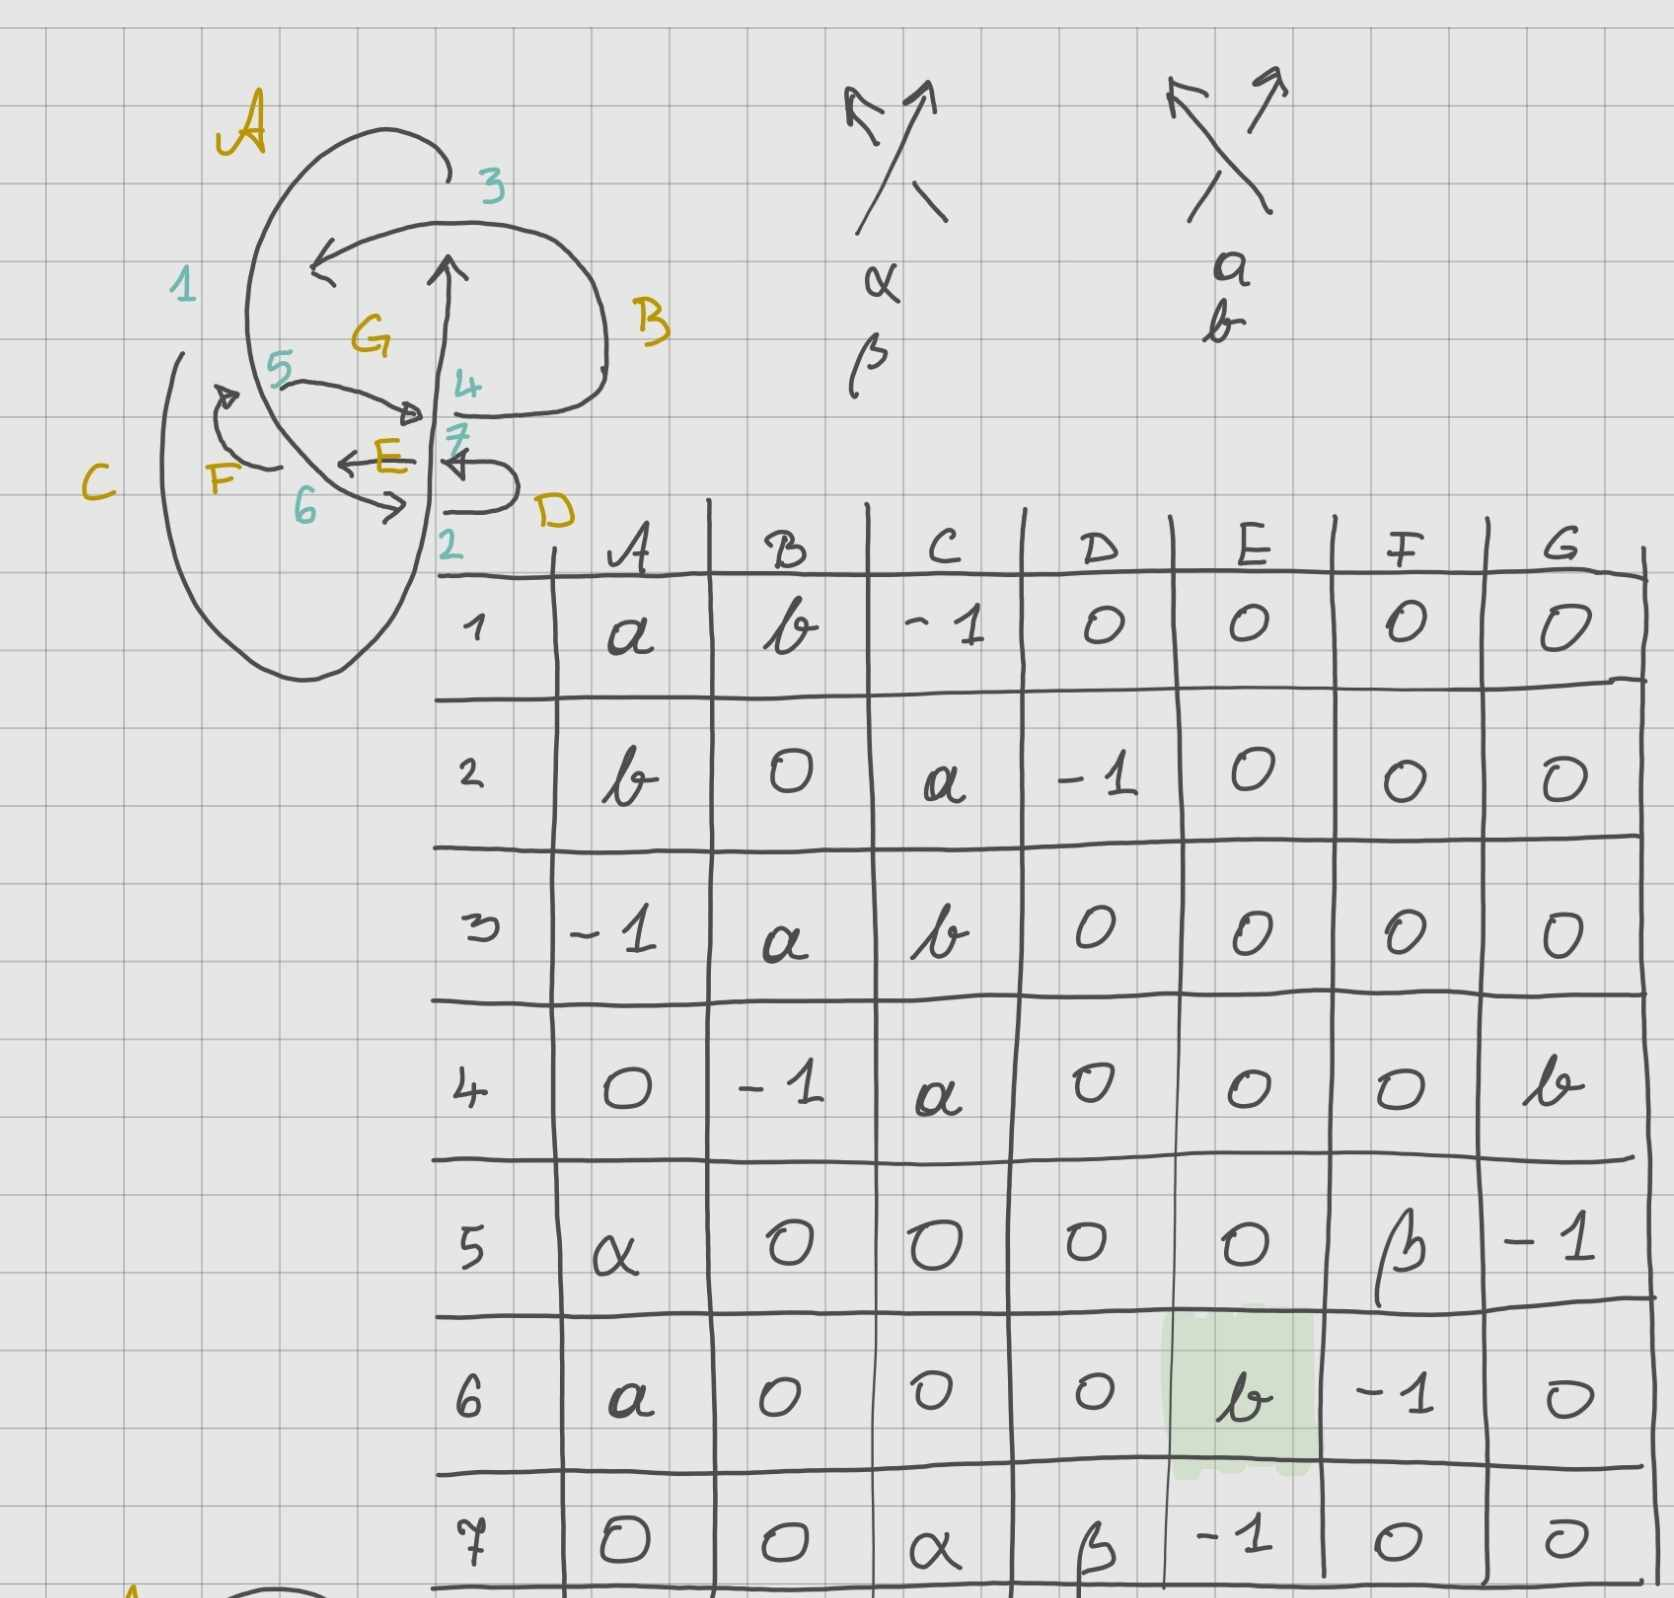
\includegraphics[width=\textwidth]{./rozdzialy/relacja_trefl_3.jpg}

  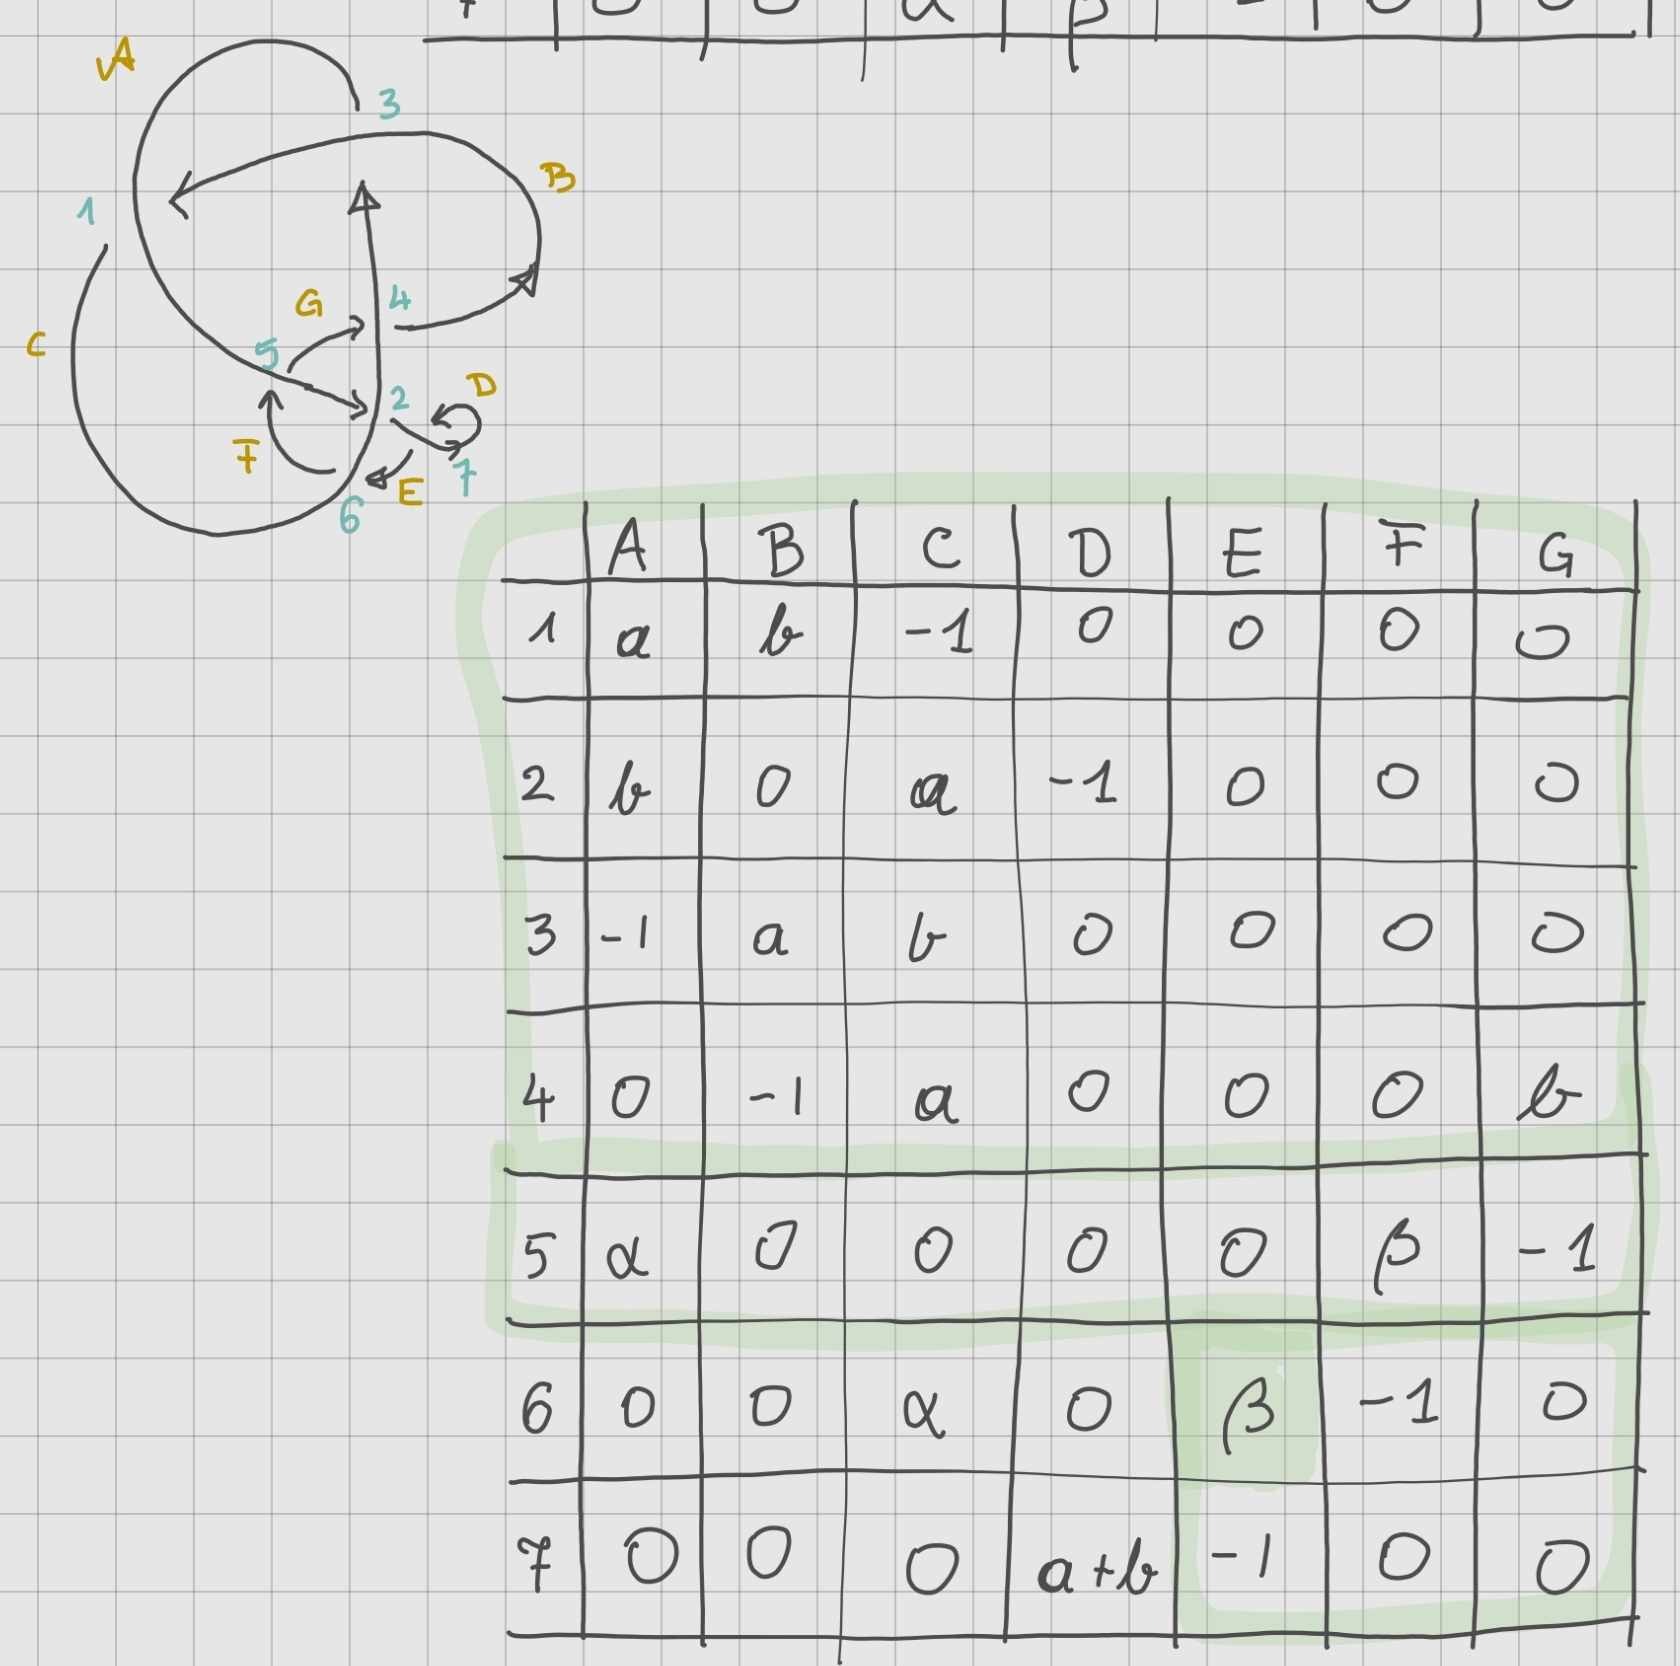
\includegraphics[width=\textwidth] {./rozdzialy/relacja_trefl_4.jpg}
\end{center}

\section{Troszkę grafu Gaussa}

\begin{center}
  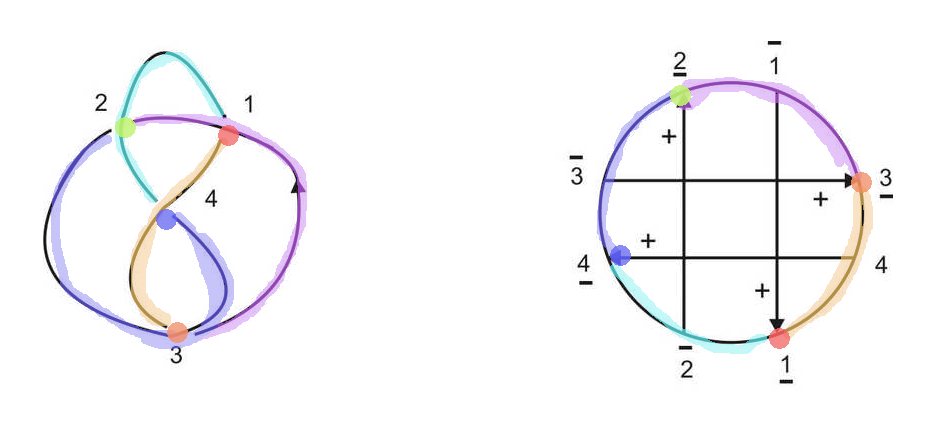
\includegraphics[width=\textwidth]{./rozdzialy/gauss_test.png}
\end{center}

Łuczki między grotami strzałek w grafie Gaussa odpowiadają łuczkom w grafie Reidemeistera.

To, gdzie idzie strzałka zaczynająca się gdzieś na łuczku mówi nam, nad którymi innymi dwoma łuczkami będzie on przechodził i w jakiej kolejności.

Nie wiem do końca jak będzie wtedy wyglądał kink.

To jedyna obserwacja jaką do tej pory miałam.


% \section*{Plan działania}

\begin{enumerate}
  \item Relacje na macierzach -> Reidemeister
    \begin{enumerate}
      \item propagation rule - funkcja $\phi$, potencjalnie dla uproszczenia będziemy pisać $\phi_+$ i $\phi_-$ na reguły kolorowania dwóch typów skrzyżowania
      \item Diagram, s łuczków i x skrzyżowań - macierz która bardzo nie jest niezmiennikiem węzła, a zależy od diagramu.
      \item Wprowadzamy relację na zorientowanych diagramach (chociaż w sumie chyba nie potrzebuję orientacji, ale na takich pracuję więc elo)
    \end{enumerate}
  \item Smith normal form 
  \item Skein relations
  \item moduł Alexandera $6_1$ i $9{46}$, czy są różne
  \item rezolwenty
  \item zmiana pidów
\end{enumerate}


\newpage

\tableofcontents

\newpage

\section{Introduction}

{\large\color{red}KTO CO ROBIŁ}

In mathematical terms, a knot is a particular embedding $S^1\hookrightarrow S^3$. A knot diagram is a projection $D:S^1\twoheadrightarrow \R^2$ along a vector such that no three points of the knot lay on this vector \cite{likorish-diagram}.

$S^1$ is an orientable space thus we can choose an orientation for a knot being considered. Then a diagram $D$ is oriented if it is a projection of an oriented $S^1$.

Intuitively, two knots $K_1$ and $K_2$ are equivalent if we can deform one into the other without cutting it and only manipulating it with our hands \cite{murasagi-equivalence}. This translates to equivalence of diagrams, which is generated by a set of moves, called the \buff{Reidemeister moves}. In the case of a diagram without an orientation, three moves are sufficient. When an orientation is imposed on $D$, at least $4$ moves are required \cite{ruchy_zorientowane}.

\section{What is a knot coloring}

Let $K$ be a knot and $D$ be its oriented diagram with $s$ segments and $x$ crossings. In such diagrams we can see two different crossing types as seen in \cref{crossing_type}. 
\begin{figure}[h]\centering
  \begin{tikzpicture}
    \draw[->] (0,0) node[below] {i} -- (1.5, 2) node[above] {o};
    \fill[white] (0.75, 1) circle (6pt);
    \draw[->] (1.5, 0)--(0, 2) node[above] {u};
    \node at (0.75, -0.5) {$+$};

    \draw[->] (4.5, 0) node[below] {i} --(3, 2) node[above] {o};
    \fill[white] (3.75, 1) circle (6pt);
    \draw[->] (3, 0)--(4.5, 2) node[above] {u};
    \node at (3.75, -0.5) {$-$};
  \end{tikzpicture}
  \caption{Two types of crossing in oriented diagram.\label{crossing_type}}
\end{figure}

Take a commutative ring with unity $R$ and an $R$-module $M$.

\begin{definition}[coloring rule]
  Take $\mathcal{C}\subseteq M^3$ to be a finitely generated submodule of $M^3$. We will call $\mathcal{C}$ a \buff{coloring rule}. There are two submodules $\mathcal{C}_\pm\subseteq \mathcal{C}$, each corresponding to a type of crossing in diagram $D$. 
\end{definition}

We can now construct three homomorphisms
$$\phi:M^3\to M/\mathcal{C}=N$$
$$\phi_\pm:M^3\to M/\mathcal{C}_\pm=N_\pm.$$
We will call $\phi$ and $\mathcal{C}$ \buff{coloring rule} interchangeably.

%Take a commutative ring with unity $R$ and two $R$-modules $M$ and $N$. Take two arbitrary module homomorphisms $\phi_+:M^3\to N$ and $\phi_-:M^3\to N$, one for each type of crossing.

% \begin{definition}[diagram coloring]
%   Let $x_1,..., x_s\in M$ be labels of arcs in diagram $D$. We will say that $(x_1,...,x_s)\in M^s$ is a \buff{coloring} if for every crossing $\pm$ in $D$ consisting of arcs $u$, $i$, $o$ the following relation is satisfied
%   $$\phi_\pm(u,i,o)=0.$$
% \end{definition}

For each crossing $x_j$ in diagram $D$ we can construct a projection 
$$\pi_{x_j}:M^s\twoheadrightarrow M^3$$
which restricts $M^s$ to the three arcs that constitute $x_j$.

\begin{definition}[diagram coloring]
  A \buff{coloring of diagram} $D$ is any element $(m_1,..., m_s)\in M^s$ that assigns elements of $M$ to each arc. We will call this coloring \buff{admissible} if for every crossing $x_j$ of type $\pm$ we have 
  $$\pi_{x_j}(m_1,..., m_s)\in \mathcal{C}_\pm\subseteq\mathcal{C}.$$
\end{definition}

% It is easy to express admissibility of a coloring in terms of homomorphism $\phi$.

It will be beneficial to express admissibility of a coloring in terms of homomorphism $\phi$.
\begin{proposition}
  A coloring $(m_1,..., m_s)\in M^s$ is a admissible $\iff$ for each crossing $x_j$ of type $\pm$ 
  $$\phi_\pm(\pi_{x_j}(m_1,...,m_s))=0.$$
\end{proposition}

\begin{proof}
  Stems from the fact that $\mathcal{C}_\pm=\ker\phi_\pm$.
\end{proof}

% \begin{definition}[diagram coloring]
%   Let $x_1,..., x_s\in M$ be labels of arcs in diagram $D$. We will say that $(x_1,...,x_s)\in M^s$ is a \buff{coloring} if for every crossing $\pm$ in $D$ consisting of arcs $u$, $i$, $o$ the following relation is satisfied
%   $$\phi_\pm(u,i,o)=0.$$
% \end{definition}

% Every crossing in the colored diagram $D$ of knot $K$ yields $x$ relations $\phi_\pm(u,i,o)=0$ which we might treat as linear equations of form 
% $$\phi_+(u,i,o)=au+bi+co=0,$$
% $$\phi_-(u,i,o)=\alpha u+ \beta i+ \gamma o=0,$$
% where $u$, $i$ and $o$ are labels assigned to arcs entering some crossing and $a,b,c\in\Hom(M, N)$.
%
% \begin{definition}
%   Matrix $D\phi:M^s\to N^x$ of coefficients taken from relations $\phi_\pm(u,i,o)$ will be called a \buff{color checking matrix}. 
%   %such that every row has only $3$ nonzero terms, corresponding to arcs entering the appropriate crossing. If $\phi_\pm(u,i,o)=a_\pm u+b_\pm i+c_\pm o$ then those terms will be $a_\pm$, $b_\pm$ and $c_\pm$.
% \end{definition}
%
% Notice that $(x_1,..., x_s)$ is a coloring of the diagram $D$ if and only if it is an element of $\ker D\phi$. However, we can choose $\phi$ to have only a trivial kernel, then only one coloring is admissible - assigning a $0$ to every arc of $D$. Thus, to obtain valuable information about the knot $K$ whose diagram is being colored, we must impose the following restrictions on $\phi$.
% %a knot invariant we must impose some restrictions on $\phi$.

\begin{definition}[color checking matrix]
  After assignings arcs to coordinates in $M^s$ and crossings to coordinates in $N^x$ it is possible to define a linear homomorphism $D\phi:M^s\to N^x$  as
  $$D\phi(m_1,...,m_s)=(\phi_\pm(\pi_{x_1}(m_1,...,m_s)), \phi_\pm(\pi_{x_2}(m_1,...,m_s)),...).$$
  Matrix that is created after choosing a basis for $M^s$ and $N^x$ will be called a \buff{color checking matrix}.
\end{definition}

Taking $\phi_\pm$ to be linear equations of form
$$\phi_+(u,i,o)=au+bi+co$$
$$\phi_-(u,i,o)=\alpha u+\beta i+\gamma o,$$
where $u$, $i$ and $o$ correspond to arcs as seen in \cref{crossing_type} and all the coefficients are linear homomorphisms $M\to N$, we know that all the entries for the color checking matrix will be linear combinations of $a$, $b$, $c$, $\alpha$, $\beta$, $\gamma$. If $M$ has $n$ generators we chose to block the matrix $D\phi$ into $n\times n$ blocks.

\begin{proposition}
  Coloring $(m_1,...,m_s)\in M^s$ is admissible $\iff$ $(m_1,...,m_s)\in\ker D\phi$.
\end{proposition}

\begin{proof}\color{blue}
  $\implies$

  We know that every projection $\pi_{x_j}(m_1,...,m_s)$ is in $\ker\phi_\pm$, depending on the type of $x_j$ crossing. Thus, there is no projection $\pi_{x_j}$ that is not being reduced by $\phi_\pm$.

  $\impliedby$

\end{proof}

{\color{blue}We need to impose restrictions on the coloring rule.} We want $\mathcal{C}$ to be two dimensional (have two generators). That way we have the following diagram
% \begin{center}
% \begin{tikzcd}
%   M^2 & M^3\arrow[l, twoheadrightarrow] \arrow[r, hookleftarrow] & \mathcal{C}\arrow[ll, bend left=20, red, "\sim"]
% \end{tikzcd}
% \end{center}
\begin{center}
\begin{tikzcd}
  M^2 \arrow[r, hookrightarrow] \arrow[rr, bend right=20, red, "\sim" below] & M^3 \arrow[r, twoheadrightarrow] & \mathcal{C}
\end{tikzcd}
\end{center}
We can assume that $M^2$ corresponds to the 'up' and 'in' segments in a crossing (compare \cref{crossing_type}), then we can define $\phi_\pm'$ to take $u$ and $i$ segments and return the out segment so that the labeling agrees with the coloring rule. Now, take the red arrow in the diagram above to be the correspondence
$$(u, i)\mapsto (u, i, \phi_\pm'(u,i)).$$
This demands that both $c$ and $\gamma$ in the definition of $\phi_+$ and $\phi_-$ are invertible. For the sake of simplicity, we will take $c=\gamma=-1$. 

With this assumption for any admissible coloring $(u,i,o)$ of a crossing we have the following relation:
$$\phi_+\;:\;o=au+bi$$
$$\phi_-\;:\;o=\alpha u+\beta i.$$


%it will be beneficial to demand that the red arrow is an isomorphism.
% \begin{enumerate}
%   \item To allow \emph{trivial colorings}, that is colorings in which every arc is assigned the same value it is necessary that
%     $$(\forall\;m\in M)\;\phi_\pm(m,m,m)=0.$$
%   \item To simplify operations of color checking matrices, if
%     $$\phi_+(u, i, o)=au+bi+co$$
%     $$\phi_-(u,i,o)=\alpha u+\beta i+\gamma o,$$
%     then we take $c$ and $\gamma$ to be invertible. For the sake of simplicity, take $c=\gamma=-1$.
%   \item The two variations of orientation of the first Reidemeister move, pictured in \cref{fig: ograniczanie phi reidemeister 1}, put the following constrictions on $a$, $b$ and $\alpha$, $\beta$:
%     $$\begin{cases}
%       a+b=1\\
%       \alpha+\beta=1
%     \end{cases}$$
%   \item Lastly, from the second Reidemeister move, pictured in \cref{fig: ograniczanie phi reidemeister}, one can gather that  
%     $$\begin{cases}
%       a+b\alpha=0\\ 
%       b\beta=1
%     \end{cases}$$
%     meaning that both $b$ and $\beta$ must be units.
% \end{enumerate}
% %
% \begin{figure}[h]\centering
%   \begin{tikzpicture}
%       \begin{knot}[
%         clip width=20pt, 
%         consider self intersections,
%         flip crossing=1
%         ]
%         \strand[thick, ->] (0, 0) to[out=90, in=-90] (0, 1) to[out=90, in=150] (1, 2.5) to[out=-30, in=90] (1.3, 2) to[out=-90, in=30] (1, 1.5) to[out=-150, in=-90] (0, 3) to[out=90, in=-90] (0, 4);
%
%         \strand[thick, ->] (3, 0)--(3, 4);
%
%       \end{knot}
%       \draw[dashed, <->] (1.5, 2)--(2.7, 2);
%
%       \node at (-.5, 2) {$+$};
%       \node at (-1.3, 3.7) {$(a+b)x $};
%       \node at (-.3, -.3) {$x$};
%       \node at (3.3, -.3) {$x$};
%     \begin{scope}[shift={(0, -6)}]
%       \begin{knot}[
%         clip width=20pt, 
%         consider self intersections
%         ]
%         \strand[thick, ->] (0, 0) to[out=90, in=-90] (0, 1) to[out=90, in=150] (1, 2.5) to[out=-30, in=90] (1.3, 2) to[out=-90, in=30] (1, 1.5) to[out=-150, in=-90] (0, 3) to[out=90, in=-90] (0, 4);
%
%         \strand[thick, ->] (3, 0)--(3, 4);
%
%       \end{knot}
%       \draw[dashed, <->] (1.5, 2)--(2.7, 2);
%       \node at (-.5, 2) {$-$};
%
%       \node at (-1.3, 3.7) {$(\alpha+\beta)x $};
%       \node at (-.3, -.3) {$x$};
%       \node at (3.3, -.3) {$x$};
%     \end{scope}
%   \end{tikzpicture}
%   \caption{The two variations of the first Reidemeister move in oriented diagrams. They suggest that $(a+b)=1$ and $(\alpha+\beta)=1$.\label{fig: ograniczanie phi reidemeister 1}}
% \end{figure}
%
% \begin{figure}[h]\centering
%   \begin{tikzpicture}
%     \begin{knot}[
%       clip width=20pt, 
%       flip crossing=1,
%       flip crossing=2
%       ]
%       \strand[thick, ->] (0,-1)--(0, 4);
%       \strand[thick, ->] (-1, -1) to[out=90, in=180+45] (-.8, 0) to[out=45, in=-90] (1, 1.5) to[out=90, in=-45] (-.8, 3) to[out=180-45, in=-90] (-1, 4);
%
%       \strand[thick, ->] (5, -1) -- (5, 4);
%       \strand[thick, ->] (6, -1) -- (6, 4);
%
%     \end{knot}
%     \draw[dashed, <->] (1.5, 1.5)--(4.5, 1.5);
%
%     \node at (-1.3, -.3) {$x$};
%     \node at (.3, -.3) {$y$};
%     \node[anchor=east] at (-.3, 1.5) {$\alpha x+\beta y$};
%     \node[anchor=west] at (.3, 3.7) {$(a+b\alpha) x+b\beta y$};
%
%     \node at (4.7, -.3) {$x$};
%     \node at (6.3, -.3) {$y$};
%
%   \end{tikzpicture}
%   \caption{Second Reidemeister move. It suggests that $(a+b\alpha)=0$ and $b\beta =1$.\label{fig: ograniczanie phi reidemeister}}
% \end{figure}
%
%
% \marginnote{jeszcze przemyśleć tekst}
% It is worth mentioning that examining the second Reidemeister move (\cref{fig: ograniczanie phi reidemeister}) with $\phi_\pm$ changed to $2\times 2$ matrices $A_\pm$, which take arcs entering a crossing as input and output the arcs leaving it, we can see that 
% $$A_+ A_-=\begin{bmatrix}0 & 1\\ b & a\end{bmatrix}\begin{bmatrix}\alpha & \beta \\ 1 & 0\end{bmatrix}=Id.$$
% This means that from homomorphism $\phi_+$ we are able to calculate $\phi_-$ and vice versa.
%
% The color checking matrix is not a knot invariant, despite the restrictions laid on $\phi$. Changing the number of crossings in a diagram will obviously create a different matrix for the same knot. We will thus proceed to define an equivalence relation on the set of all color checking matrices of a knot $K$.

% Let $R$ be a commutative ring, typically $\Z[\Z]$, and take $M,N$ to be two $R$-modules. Consider two module homomorphisms $\phi_+:M^3\to N$ and $\phi_-:M^3\to N$ such that
% $$(\forall\;x\in M)\;\phi_\pm(x,x,x)=0.$$ 
% This homomorphism will be used to determine whether or not a labelling of knot arcs constitutes a coloring or not.
%
% \medskip
%
%
% {\large\color{red}tak naprawdę wystarczy jeden homomorfizm $\phi$, ale nie wiem jeszcze jak to wyjaśnić beż zahaczania o linki lub warkocze}.
% %{\large\color{red}JAK WUTLUMACZYC, ZE NAPRAWDE TO WYSTARCZY JEDNA FUNKCJA, ALE TAK BEDZIE MI LATWIEJ W ZYCIU? BO JAK NARYSUJĘ DIAGRAM Z DWOMA SKRZYŻOWANIAMI JEDNO + A DRUGIE - I POŁĄCZĘ JAK PRZY WARKOCZE -> LINKI TO DOSTAJĘ LINKA Z 2 KOMPONENTAMI :V}
% % It might appear that in the case of oriented diagram two different functions $\phi$ are required. However, considering the following diagram
% % \begin{figure}[h]\centering 
% %   \begin{tikzpicture}
% %     \draw[->] (0,-0.5) to (0, -1) to [out=-90, in=90] (1, -3);
% %     \draw[->] (1, -3) to (1, -3.5) to[out=-90, in=90] (0, -5.5) to (0,-6);
% %
% %     \fill[white] (.5, -2) circle (6pt);
% %     \fill[white] (.5, -4.5) circle (6pt);
% %
% %     \draw[->] (1,-0.5) to (1, -1) to[out=-90, in=90] (0, -3);
% %     \draw[->] (0, -3) to (0, -3.5) to[out=-90, in=90] (1, -5.5) to (1, -6);
% %     \draw (1, -6) to [out=-90, in=-90] (3, -4) to[out=90, in=-90] (3, -2.5) to[out=90, in=90] (1, -.5);
% %
% %     \node at (1, -2) {$-$};
% %     \node at (1, -4.5) {$+$};
% %   \end{tikzpicture}
% %   \caption{Why only one function $\phi$ is required?\label{just_why_phi}}
% % \end{figure}
%
% \medskip
%
%
% The color checking matrix in itself is obviously not a knot invariant. However, we might define an equivalence relation on the set of all matrices $M^m\to N^n$, $m,n\in\N$, such that all the matrices which come from the same knot fall into the same equivalence class.
%



We might also demand that a trivial coloring (every arc is assigned the same element of $M$) is an admissible coloring.

The color checking matrix is not a knot invariant. Changing the diagram with accordance to the Reidemeister moves might change the dimensions of the matrix. Thus, we need to define an equivalence relation on the set of all color checking matrices.


\subsection{Relation on color checking matrices}

In order to ensure that all matrices that stem from the same knot are considered in one equivalence class we will look at how Reidemeister moves change the matrix. 

In this section we will always assume that the diagram labeled as $D$ has $s$ segments and $x$ crossings. This means that always 
$$D\phi:M^s \to N^x.$$
Furthermore, we will always put rows and columns corresponding to crossings and segments that are affected by the Reidemeister move as the last columns and rows of the matrix.

\subsection*{\centering R1}

\def\bracketL{[}
\def\bracketR{]}
\renewcommand{\figurename}{}
\captionsetup{labelformat=empty}

\begin{figure}[h!]\centering 
  \caption{\textbf{R1a}\label{R1a}}
  \medskip

  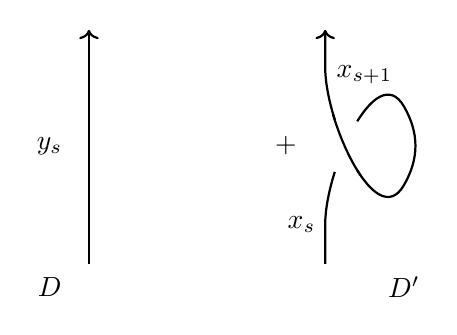
\begin{tikzpicture}
    \begin{knot}[
      consider self intersections,
      clip width=20pt,
      flip crossing=1
      ]
      \strand[->, thick] (0, -1.5) to [out=90, in=-90] 
        (0, -1) to[out=90, in=120] 
        (1, 0.5) to[out=-60, in=60] 
        (1, -0.5) to[out=-120, in=-90] 
        (0, 1) to[out=90, in=-90] (0, 1.5);

      \strand[->, thick] (-3, -1.5) -- (-3, 1.5);
    \end{knot}
    \node at (-.5, 0) {$+$};
    \node at (-3.5, -1.8) {$D$};
    \node at (1, -1.8) {$D'$};

    \node at (-3.5, 0) {$y_s$};
    \node at (-0.3, -1) {$x_s$};
    \node at (0.5, 0.9) {$x_{s+1}$};
  \end{tikzpicture}
\end{figure}

In oriented diagrams, there are four distinct Reidemeister moves \cite{ruchy_zorientowane}, the first one having to account for two types of crossing. We start with \textbf{R1a}, pictured in \cref{R1a}. Consider the two matrices 
$$D\phi:M^s\to N^x$$ 
$$D'\phi:M^{s+1}\to N^{x+1}.$$
Only two arcs change between the two, thus 
$$D\phi\restriction M^{s-1}=D'\phi\restriction M^{s-1}.$$
Furthermore, we want to assert that the two arcs $x_s$ and $x_{s+1}$, into which $y_s$ is split, are arranged in a $+$ type crossing. Thus, for all $x_s, x_{s+1}\in M$ we require that
$$\pi_{x+1}[D'\phi(0,..., x_s, x_{s+1})]=\phi_+(x_{s+1},x_s,x_{s+1}),$$
where $\pi_{x+1}$ is projection onto the last coordinate. 
Additionally, we want the column that represented contribution of the twisted arc in diagram $D$ to be the sum of two new arcs in $D'\phi$, meaning that for every $y_s\in M$:
$$(D\phi(0,..., y_s), 0)=D'\phi(0,..., y_s, y_s).$$

\begin{figure}[h!]\centering 
  \caption{\textbf{R1b}\label{R1b}}
  \medskip

  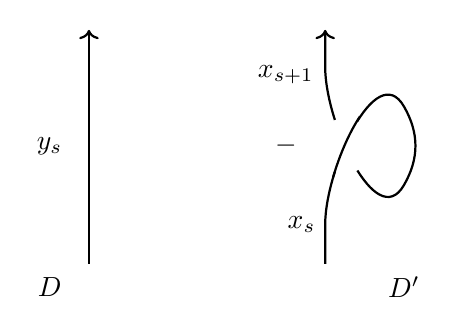
\begin{tikzpicture}
    \begin{knot}[
      consider self intersections,
      clip width=20pt
      ]
      \strand[->, thick] (0, -1.5) to [out=90, in=-90] 
        (0, -1) to[out=90, in=120] 
        (1, 0.5) to[out=-60, in=60] 
        (1, -0.5) to[out=-120, in=-90] 
        (0, 1) to[out=90, in=-90] (0, 1.5);

      \strand[->, thick] (-3, -1.5) -- (-3, 1.5);
    \end{knot}
    \node at (-.5, 0) {$-$};
    \node at (-3.5, -1.8) {$D$};
    \node at (1, -1.8) {$D'$};

    \node at (-3.5, 0) {$y_s$};
    \node at (-0.3, -1) {$x_s$};
    \node at (-0.5, 0.9) {$x_{s+1}$};
  \end{tikzpicture}

\end{figure}

The second type of \textbf{R1} is seen in \cref{R1b}. The relation for this move is almost the same as above. We start with two matrices
$$D\phi:M^s\to N^x$$
$$D'\phi:M^{s+1}\to N^{x+1}$$
that must agree on the arcs and crossings that are not changed between $D$ and $D'$:
$$D\phi\restriction M^{s-1}=D'\phi\restriction M^{s-1}.$$
The type of crossing into which an arc of $D$ is twisted in $D'$ is differented than in \textbf{R1a}, thus the second equality is slightly different: for all $x_s, x_{s+1}\in M$
$$\pi_{x+1}[D'\phi(0,..., x_s, x_{s+1})]=\phi_-(x_{s},x_s,x_{s+1}).$$
The last requirement is not changed from \textbf{R1a}, meaning that for all $y_s\in M$:
$$(D\phi(0,..., y_s), 0)=D'\phi(0,..., y_s, y_s).$$

\subsection*{\centering R2}

\begin{figure}[h!]\centering 
  \caption{\textbf{R2}\label{R2}}
  \medskip 

  \begin{tikzpicture}
    \begin{knot}[
      consider self intersections,
      clip width=20pt,
      % draft mode=crossings,
      flip crossing=1,
      flip crossing=2
      ]
      \strand[->, thick] (0.8, -2)--(.8, 2);
      \strand[->, thick] (-0.5, -2) to [out=90, in=-120] 
      (1.5, -.25) to[out=60, in=-60] 
      (1.5, .25) to[out=120, in=-90] (-.5, 2);

      \strand[->, thick] (-3, -1.5) -- (-3, 1.5);
      \strand[->, thick] (-4, -1.5)--(-4, 1.5);
    \end{knot}
    \node at (1, -1.1) {$-$};
    \node at (1, 1.1) {$+$}; 
    \node at (-4.5, -2.2) {$D$};
    \node at (1.5, -2.2) {$D'$};

    \node at (-4.6, 0) {$x_{s-1}$};
    \node at (-2.6, 0) {$x_s$};

    \node at (2.1, 0) {$x_{s-1}$};
    \node at (0.3, 0) {$x_{s+1}$}; 
    \node at (0.4, -1.8) {$x_s$};
    \node at (0.3, 1.8) {$x_{s+2}$};
  \end{tikzpicture}
\end{figure}

For this Reidemeinster move we start with matrices 
$$D\phi:M^s\to N^x$$
$$D'\phi:M^{s+2}\to N^{x+2}.$$
Only two segments of $D$ are manipulated, thus
$$D\phi\restriction M^{s-2}=D'\phi\restriction M^{s-2}.$$
To ensure that the poke contributes adequate crossings, we want for every $x,y\in M$
\begin{align*}
  &D'\phi(0,..., x,y,y,y)=\\
  =&(D\phi(0,..., x,y), \phi_-(x,y,y), \phi_+(x,y,y))
\end{align*}

\subsection*{\centering R3}

\begin{figure}[h!]\centering 
  \caption{\textbf{R3}\label{R3}}
  \medskip 

  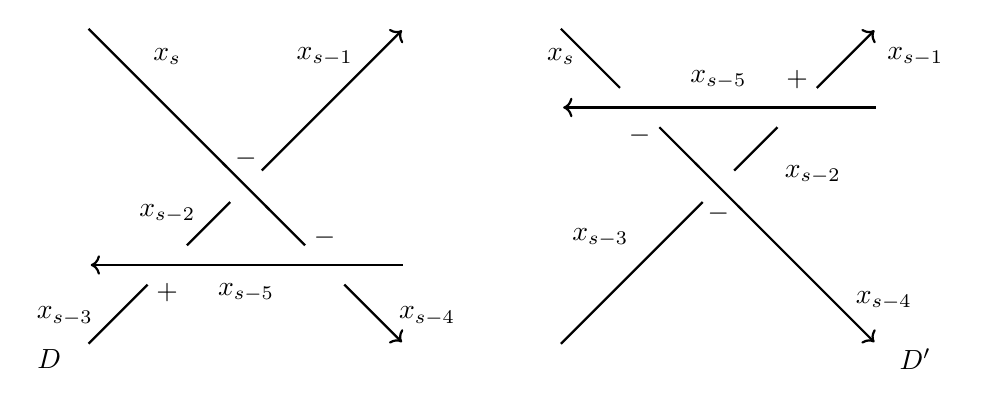
\begin{tikzpicture}
    \begin{knot}[
      consider self intersections,
      clip width=20pt,
      %draft mode=crossings,
      ignore endpoint intersections=false,
      flip crossing=1,
      flip crossing=2,
      flip crossing=3,
      flip crossing=4,
      flip crossing=5,
      flip crossing=6
      ]
      \strand[->, thick] (0, 0) to [out=45, in=-180+45] (4, 4);
      \strand[<-, thick] (4, 0) to [out=180-45, in=-45] (0, 4);
      \strand[<-, thick] (0, 1) -- (4, 1);

      \strand[->, thick] (6, 0) to [out=45, in=-180+45] (10, 4);
      \strand[<-, thick] (10, 0) to [out=180-45, in=-45] (6, 4);
      \strand[<-, thick] (6, 3) -- (10, 3);
    \end{knot}
    \node at (-0.5, -.2) {$D$};
    \node at (10.5, -.2) {$D'$};

    \node at (2, 2.35) {$-$};
    \node at (1, 0.65) {$+$};
    \node at (3, 1.35) {$-$};

    \node at (2, 0.65) {$x_{s-5}$};
    \node at (1, 3.65) {$x_{s}$};
    \node at (3, 3.65) {$x_{s-1}$};
    \node at (1, 1.65) {$x_{s-2}$};
    \node at (-0.3, 0.35) {$x_{s-3}$};
    \node at (4.3, 0.35) {$x_{s-4}$};

    \node at (8, 1.65) {$-$};
    \node at (9, 3.35) {$+$};
    \node at (7, 2.65) {$-$};

    \node at (2+6, 3.35) {$x_{s-5}$};
    \node at (6, 3.65) {$x_{s}$};
    \node at (10.5, 3.65) {$x_{s-1}$};
    \node at (9.2, 2.15) {$x_{s-2}$};
    \node at (6.5, 1.35) {$x_{s-3}$};
    \node at (4.1+6, 0.55) {$x_{s-4}$};
  \end{tikzpicture}
\end{figure}

$$D\phi\sim D'\phi$$
$$\text{if and only if}$$
\marginnote{WRÓCIĆ I DOPISAĆ?} %TO DO
\begin{align*}
  &D\phi\restriction M^{s-5}=D'\phi\restriction M^{s-5}\land \\ 
  \land & (\forall\;x,y,z\in M) \pi_{x-3}[D\phi(0,...,x,y,z)]=\\ 
        &= \pi_{x-3}[D'\phi(0,...,z,x,y,0,0)]\land \\ 
  \land & D\phi(0,...., z,y,0,0,0,x)=D'\phi(0,...,z,y,0,0,0,x)\land \\ 
  \land & D\phi(0,...,z,0,y,x,0,0) = D'\phi(0,...,z,0,0,y,x,0)
\end{align*}


\begin{theorem}
  Let $K$ be a knot and $D$ its oriented diagram. Define 
  $$K\phi:=[D\phi]$$
  to be the equivalence class of the matrix $D\phi$. Then, $K\phi$ is a knot invariant.
\end{theorem}

\begin{proof}
  An immediate result of construction presented above.\marginnote{brzydko brzmi}% TO DO
\end{proof}

\renewcommand{\figurename}{Figure}
\captionsetup{labelformat=simple}

\section{Smith normal form}

% To obtain the most general invariants, we take $R$ to be $\Z[t, t^{-1}]$, the ring of Laurent polynomials with integer coefficients. However, this ring is not a principal ideal domain 
% the ring $R$ is not a PID but $\Z[\Z]$. It is possible to find invariants over this particular ring, however it is often beneficial to find a PID ring $P$ and send $t\in \Z[\Z]$ to some unit of $P$. 
%
% % Take $P=\Q[\Z]$ and consider a matrix $A\in K\phi$ as a matrix with terms in $P$-module.
The ring $R$ over which we consider modules $M$ and $N$ is not necessary a principal ideal domain. However, there are plenty of PID rings and one can take any unit of $R$ and send it to any unit of a PID ring $P$ to allow for $M$ and $N$ to be considered as $P$-modules. That way, we can consider a new type of equivalence relation on any color checking matrix $D\phi$.
\begin{definition}
Take $A\in K\phi$ and consider it as a $s\times x$ matrix with terms in a $P$-module $M$. Then there exist a $s\times s$ matrix $S$ and $x\times x$ matrix $T$ such that $SAT$ is of form
$$
\begin{bmatrix}
  a_1 & 0 & 0 & \hdots & 0 & \hdots & 0 \\ 
  0 & a_2 & 0\\ 
  0 & 0 & \ddots & & \vdots & & \vdots\\ 
  \vdots & & & a_r\\ 
  0 & & \hdots & & 0 & \hdots & 0 \\ 
  \vdots & & & & \vdots & & \vdots\\ 
  0 & & \hdots & & 0 & \hdots & 0
\end{bmatrix}
$$
where for every $i$ $a_i|a_{i+1}$. Such matrix $SAT$ is called \textbf{Smith normal form} of matrix $A$.
\end{definition}
{\color{blue}
To obtain the most general invariants, we take $R$ to be $\Z[t, t^{-1}]$, the ring of Laurent polynomials with integer coefficients. There are multitudes of PIDs $P$ with homomorphisms $\Z[t, t^{-1}]\to P$.
}

{
  \color{red}\large 
  DOPISAĆ JAKIE OPERACJE ŻEBY DOSTAĆ ŁOPATOLOGICZNIE SMITH NORMAL FORM
}

As was mentioned in the first section, $\overline{x}\in M^s$ is a coloring of a diagram $D$ if and only if $D\phi(\overline{x})=0$, that is $\overline{x}\in\ker D\phi$. The Smith normal form hints at the structure of matrix kernel - the columns filled with zeros will contributed a free factor $M$ to the kernel. 

Take $(a)$ to be a prime ideal with its generator $a$ appearing in the Smith normal form of $D\phi$. Then we might consider the matrix over a new ring $R/(a)$, which is still a PID. After this change, the structure of the kernel has changed as now there are additional zero columns where $a$ and all its multiples stood.

\begin{definition}[reduced normal form of matrix]
  Take $A$ to be a matrix with coefficients in principal ideal domain $P$. Take $a_1,...,a_k\in P$ to be all the elements of the Smith normal form of $A$ that are neither zero nor invertible. Consider a new square matrix 
  $$
  \begin{bmatrix}
    a_1 & 0 & 0 & \hdots & 0\\ 
    0 & a_2 & 0 & \hdots & 0 \\ 
    0 & 0 & \ddots & &  \\ 
    \vdots & \vdots & & & \vdots \\ 
    0 & 0 & \hdots & 0 & a_k
  \end{bmatrix}
  $$
  which will be called the \buff{reduced normal form} of matrix $A$.
\end{definition}

The following example justifies the utility of the reduced normal form of color checking matrices in distinguishing knots.

\begin{example} 
  Consider the knots $6_1$ with diagram as seen in \cref{fig:6_1:knot} and $9_{46}$ pictured in \cref{fig:9_46:knot}, ring $R=\Z[t, t^{-1}]$, $M=R$ and 
  $$\begin{cases}
    \phi_+(u, i, o)=(1-t)u+ti-o\\ 
    \phi_-(u,i,o)=(1-t^{-1})u+t^{-1}i-o.
  \end{cases}$$ 
  The two rings have the same Alexander polynomial, $\Delta=-2t^{-2}+5t^{-1}-2$, and the same Alexander module $H^1(S^3-K)=\Z[t, t^{-1}]/(\Delta)$.


  For the knot $6_1$ we find the matrix $D\phi$ and after changing to the $PID$ ring $P=\Q[t, t^{-1}]$ we see that the Smith normal form is:
\begin{figure}[h]\centering
  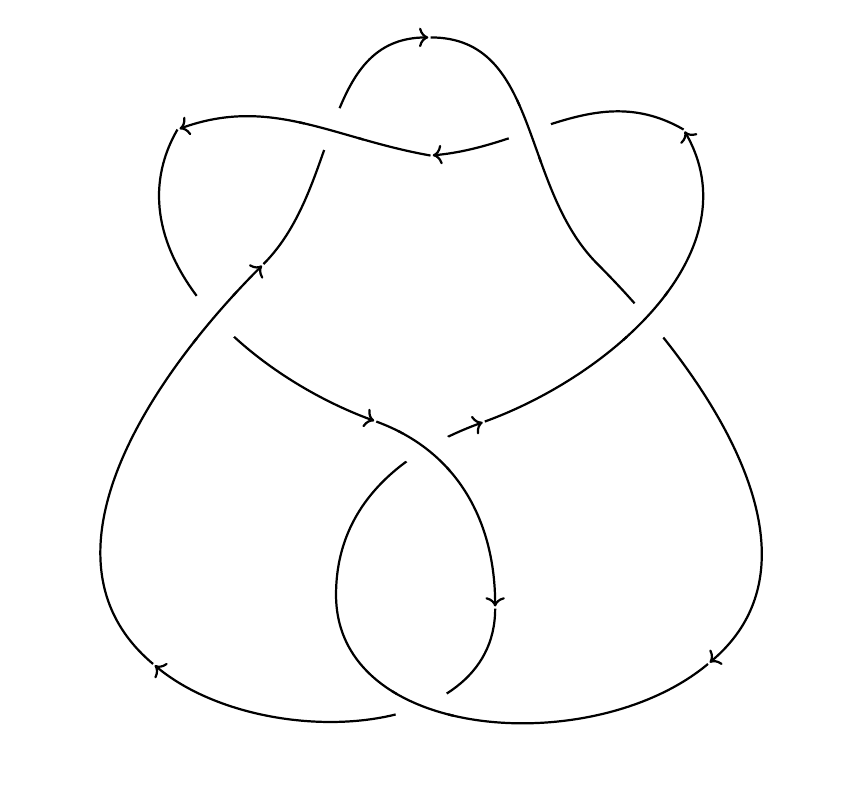
\begin{tikzpicture}[bgnd/.style={circle, fill=white, draw=white}]
    %\node[opacity=0.2] at (0,0) {\includegraphics[width=0.7\textwidth]{./rozdzialy/6_1-3d.png}};

    \coordinate (a0) at (0,0);
    \coordinate (a1) at (90:5);
    \coordinate (a2) at (45:3);
    \coordinate (a3) at (-40:4.6);
    \coordinate (a4) at (-120:2.4);
    \coordinate (a5) at (10:0.7);
    \coordinate (a6) at (50:5);
    \coordinate (a7) at (90:3.5);
    \coordinate (a8) at (180-50:5);
    \coordinate (a9) at (170:0.7);
    \coordinate (a10) at (-70:2.4);
    \coordinate (a11) at (220:4.6);
    \coordinate (a12) at (180-45:3);

    %\foreach \i in {0,...,12} \fill (a\i) circle (2pt);

    \begin{knot}[
      clip width=20, 
      flip crossing=1,
      flip crossing=3,
      flip crossing=6
      ]
      \strand[thick, ->] (a1) to[out=0, in=90+45] (a2) to[out=-45, in=40] (a3);
      \strand[thick, ->] (a3) to[out=220, in=-90] (a4) to[out=90, in=200] (a5);
      \strand[thick, ->] (a5) to[out=20, in=-60] (a6);
      \strand[thick, ->] (a6) to[out=150, in=5] (a7);
      \strand[thick, ->] (a7) to[out=170, in=20] (a8);
      \strand[thick, ->] (a8) to[out=240, in=160] (a9);
      \strand[thick, ->] (a9) to[out=-20, in=90] (a10);
      \strand[thick, ->] (a10) to[out=-90, in=-40] (a11);
      \strand[thick, ->] (a11) to[out=140, in=180+45] (a12);
      \strand[thick, ->] (a12) to[out=45, in=180] (a1);
    \end{knot}

    %\node at (80: 5) {$A$};
    %\node at (-40:4) {$B$};
    %\node at (45:5.5) {$C$};
    %\node at (135:5.5) {$D$};
    %\node at (-1.5,0.1) {$E$};
    %\node at (220:4) {$F$};
    %
    %\node[bgnd] at (70:4.7) {$1$};
    %\node[bgnd] at (25:3.9) {$2$};
    %\node[bgnd] at (-90:3) {$3$};
    %\node[bgnd] at (90:0.5) {$4$};
    %\node[bgnd] at (110:4.7) {$5$};
    %\node[bgnd] at (180-25:3.9) {$6$};

    %\draw[dashed] (70: 4) circle (0.4);
    %\draw[dashed] (28: 3.1) circle (0.4);
    %\draw[dashed] (-90:3.5) circle (0.4);
    %\draw[dashed] (-90:0.15) circle (0.4);
    %\draw[dashed] (180-28:3.1) circle (0.4);
    %\draw[dashed] (110:4) circle (0.4);
  \end{tikzpicture}
  \caption{\label{fig:6_1:knot}Diagram of knot $6_1$.}
\end{figure}
$$A=\begin{pmatrix}
  -1 & 0 & 0 & 0 & 0 & 0 \\ 
  0 & -1 & 0 & 0 & 0 & 0 \\ 
  0 & 0 & t & 0 & 0 & 0 \\ 
  0 & 0 & 0 & t & 0 & 0 \\ 
  0 & 0 & 0 & 0 & -2t^{-2}+5t^{-1}-2 & 0 \\ 
  0 & 0 & 0 & 0 & 0 & 0 
\end{pmatrix}$$
which after reduction is
$$A'=
\begin{pmatrix}
  -2t^{-2}+5t^{-1}-2
\end{pmatrix}
$$
a $1\times 1$ matrix with the only term being the Alexander polynomial of $6_1$.

Using diagram in \cref{fig:9_46:knot} of $9_{46}$ it can be calculated that the Smith normal form of $D\phi$ is
\begin{figure}[h]\centering
  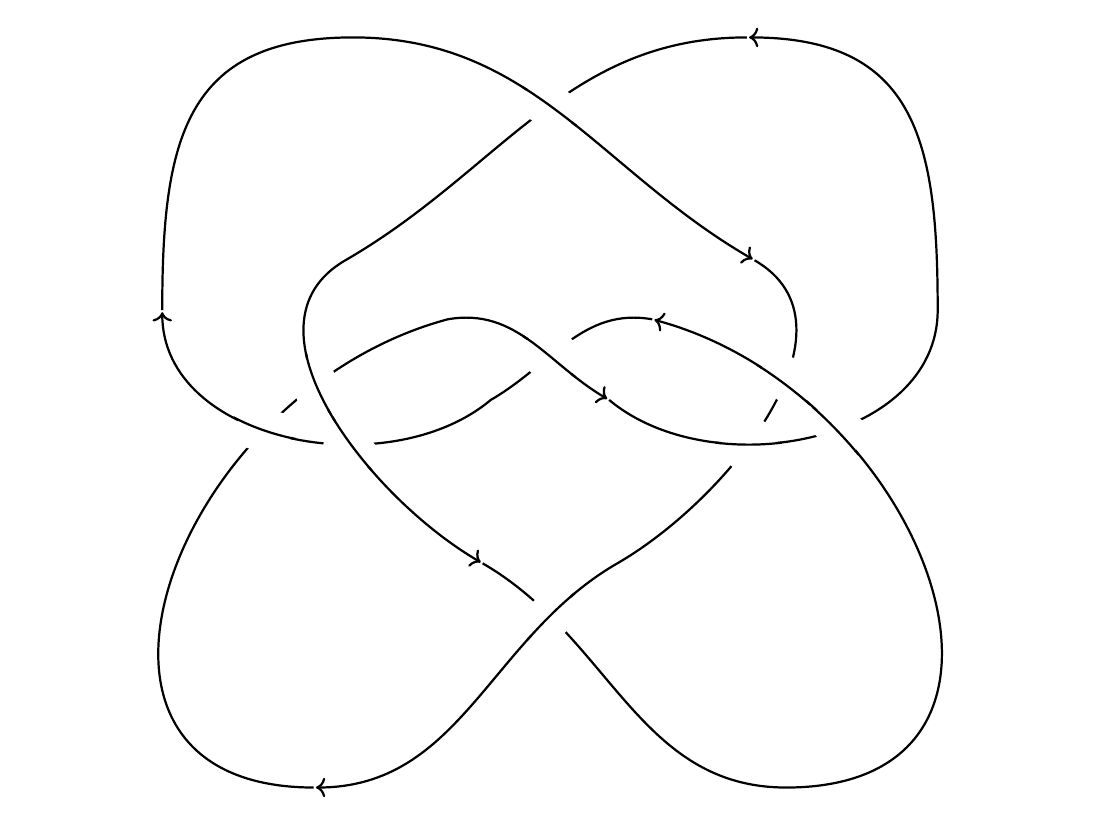
\begin{tikzpicture}[bgnd/.style={circle, fill=white, draw=white}]
    %\node[opacity=0.2] at (0,0) {\includegraphics[width=0.7\textwidth]{./rozdzialy/6_1-3d.png}};

    \coordinate (a0) at (0,0);
    \coordinate (a1) at (60:5);
    \coordinate (a2) at (150:3);
    \coordinate (a3) at (-110:2.5);
    \coordinate (a4) at (-60:6);
    \coordinate (a5) at (30:1.5);
    \coordinate (a6) at (200:0.8);
    \coordinate (a7) at (170:5);
    \coordinate (a8) at (120:5);
    \coordinate (a9) at (30:3);
    \coordinate (a10) at (-70:2.5);
    \coordinate (a11) at (180+60:6);
    \coordinate (a12) at (150:1.5);
    \coordinate (a13) at (-20:0.8);
    \coordinate (a14) at (10:5);

    %\foreach \i in {0,...,14} \fill (a\i) circle (2pt);

    \begin{knot}[
      clip width=20, 
      consider self intersections,
      ignore endpoint intersections=false,
      %draft mode=crossings,
      flip crossing=1,
      flip crossing=4,
      flip crossing=7, 
      flip crossing=9
      ]
      \strand[thick, ->] 
        (a1) to [out=180, in=30]
        (a2) to [out=210, in=150]
        (a3);
      \strand[thick, ->]
        (a3) to [out=-30, in=180] 
        (a4) to [out=0, in=-15, looseness=1.5] 
        (a5);
      \strand[thick, ->]
        (a5) to [out=170, in=30] 
        (a6) to [out=220, in=-90] 
        (a7);
      \strand[thick, ->]
        (a7) to [out=90, in=180, looseness=1.3] 
        (a8) to [out=0, in=150] 
        (a9);
      \strand[thick, ->]
        (a9) to [out=-30, in=30]
        (a10) to [out=210, in=0] 
        (a11);
      \strand[thick, ->]
        (a11) to [out=180, in=180+15, looseness=1.5] 
        (a12) to [out=10, in=150]
        (a13);
      \strand[thick, ->]
        (a13) to [out=-40, in=-90]
        (a14) to [out=90, in=0, looseness=1.3]
        (a1);
      \fill[yellow] (-10:3.7) circle (6pt);
    \end{knot}
  \end{tikzpicture}
  \caption{\label{fig:9_46:knot}Diagram of knot $9_{46}$.}
\end{figure}
$$B=\begin{pmatrix}
  1 & 0 & 0 & 0 & 0 & 0 & 0 & 0 & 0 \\ 
  0 & t^{-1} & 0 & 0 & 0 & 0 & 0 & 0 & 0 \\ 
  0 & 0 & t^{-1} & 0 & 0 & 0 & 0 & 0 & 0\\ 
  0 & 0 & 0 & t  & 0 & 0 & 0 & 0 & 0 \\ 
  0 & 0 & 0 & 0 & t  & 0 & 0 & 0 & 0 \\ 
  0 & 0 & 0 & 0 & 0 & t  & 0 & 0 & 0\\ 
  0 & 0 & 0 & 0 & 0 & 0 & 2t-t^2 & 0 & 0 \\ 
  0 & 0 & 0 & 0 & 0 & 0 & 0 & t^{-2}-2t^{-1} & 0\\ 
  0 & 0 & 0 & 0 & 0 & 0 & 0 & 0 & 0
\end{pmatrix},$$
while reduced normal form of $D\phi$ is
$$B'=
\begin{pmatrix}
  2t-t^2 & 0 \\ 
  0      & t^{-2}-2t^{-1}
\end{pmatrix}
$$
which is significantly different than the one for $6_1$. Observe also that the determinant of both matrices is equal to the Alexander polynomial of corresponding knots 
$$\det(A')=-2+5t^{-1}-2t^{-2}$$
$$\det(B')=(2t-t^2)(t^{-2}-2t^{-1})=2t+2+2t^{-1}=-t(-2+5t^{-1}-2t^{-2}).$$
\end{example}

% {\large\color{red}TO DO: sprawdzić te węzły wyżej za pomocą pow. Seiferta, czy mają różne moduły Alexandera}

\begin{theorem}
  The reduced normal form of color checking matrix does not depend on the choice of diagram $D$. Thus, it is well defined for $K\phi$ and is a knot invariant.
\end{theorem}

\begin{proof}
  \marginnote{nie wiem, czy tutaj aż tak powinno się dokładnie mówić co i jak dodaję?} % TO DO
Take a knot $K$ and its diagram $D$ with $s$ segments and $x$ crossings. We will show that applying any Reidemeister move to this knot will not change the reduced normal form of its color checking matrix.

  \subsection*{\centering R1}

  The first Reidemeister move is split into \textbf{R1a} and \textbf{R1b}. Due to those two cases being analogous, we will focus on the move \textbf{R1a} (the proof of \textbf{R1b} is left as an exercise for the reader).

  Take $D'$ to be diagram $D$ with one arc twisted into a $+$ crossing. In opposition to the assumption in previous section, we will take the arcs and crossings that differ between those two diagrams to be on first positions. Now, the matrices $D\phi$ and $D'\phi$ are as follows
  $$
  D'\phi=
  \begin{bmatrix}
    b & a-1 & 0 & \hdots\\ 
    x_2 & y_2 & \hdots \\ 
    x_3 & y_3 \\ 
    \vdots 
  \end{bmatrix}
  $$
  $$
  D\phi=
  \begin{bmatrix}
    x_2 + y_2 & \hdots \\ 
    x_3 + y_3 \\ 
    \vdots
  \end{bmatrix}
  $$
  Adding the first column of $D'\phi$ to the second column will yield 
  $$
  D'\phi=
  \begin{bmatrix}
    b & 0 & 0 & \hdots\\ 
    x_2 & x_2+y_2 & \hdots \\ 
    x_3 & x_3+y_3 \\ 
    \vdots 
  \end{bmatrix}
  $$
  because $a+b=1$. Now we know that $b$ is a unit, thus we can easily remove the elements of the first column that are not $b$. This results in 
  $$
  D'\phi=
  \begin{bmatrix}
    b & 0 & 0 & \hdots\\ 
    0 & x_2+y_2 & \hdots \\ 
    0 & x_3+y_3 \\ 
    \vdots 
  \end{bmatrix}
  $$
  notice that the lower right portion of this matrix looks exactly like $D\phi$. The only difference is a column containing a singular unit element and thus it will be struck out when computing the reduced normal form. Thus, the reduced normal form of $D'\phi$ is the same as in $D\phi$.
  
  \subsection*{\centering R2}

  Now the diagram $D'$ is a diagram $D$ with one arc poked onto another. Once again we will put those changed arcs at the beggining of the color checking matrix to obtain following matrices:
  $$
  D'\phi=
  \begin{bmatrix}
    \alpha & \beta & -1 & 0 & \hdots \\ 
    a & 0 & b & -1  \\ 
    x_3 & u_3 & 0 & v_3 \\ 
    x_4 & u_4 & 0 & v_4 \\ 
    \vdots & & & & \ddots
  \end{bmatrix}
  $$
  $$
  D\phi= 
  \begin{bmatrix}
    x_3 & u_3 + v_3 & \hdots \\ 
    x_4 & u_4 + v_4 \\ 
    \vdots
  \end{bmatrix}
  $$
  Adding the third column of $D'\phi$ multiplied by $\alpha$ and $\beta$ to first and second column respectively we are able to reduce the first row to only zeros and $-1$. Now, adding this row to the second one creates a column with only $-1$ and zeros. We can put it as the first column:
  $$
  D'\phi=
  \begin{bmatrix}
    -1 & 0 & 0 & 0 & \hdots \\ 
    0 & a +b\alpha & 0 & -1  \\ 
    0 & x_3 & u_3 & v_3 \\ 
    0 & x_4 & u_4 & v_4 \\ 
    \vdots & & & & \ddots
  \end{bmatrix}
  $$
  Notice that $a+b\alpha=0$ and so we can transform this matrix into
  $$
  D'\phi=
  \begin{bmatrix}
    -1 & 0 & 0 & 0 & \hdots \\ 
    0 & -1 & -1 & 0  \\ 
    0 & v_3 +u_3 & v_3+u_3&  x_3 & \\ 
    0 & v_4 +u_4 & v_4+u_4 & x_4 \\ 
    \vdots & & & & \ddots
  \end{bmatrix}
  $$
  and then into 
  $$
  D'\phi=
  \begin{bmatrix}
    -1 & 0 & 0 & 0 & \hdots \\ 
    0 & -1 & 0 & 0  \\ 
    0 & 0 & v_3+u_3&  x_3 & \\ 
    0 & 0 & v_4+u_4 & x_4 \\ 
    \vdots & & & & \ddots
  \end{bmatrix}
  $$
  which obviously has the same reduced normal form as $D\phi$.

  \subsection*{\centering R3}

  $$D\phi=
  \begin{bmatrix}
    \alpha & -1 & \beta & 0 & 0 & 0 \\ 
    0 & 0 & -1 & b & 0 & a \\ 
    \beta & 0 & 0 & 0 & -1 & \alpha \\ 
    u_4 & 0 & v_4 & w_4 & x_4 & y_4
  \end{bmatrix}
  $$
  $$D'\phi=
  \begin{bmatrix}
    0 & 0 & -1 & \beta & \alpha & 0 \\ 
    \beta & 0 & 0 & 0 & -1 & \alpha \\ 
    0 & -1 & b & 0 & 0 & a\\ 
    u_4 & 0 & v_4 & w_4 & x_4 & y_4
  \end{bmatrix}
  $$

  Applying row and column operations on those matrices results in 
  $$
  D\phi=
  \begin{bmatrix}
    -1 & 0 & 0 & 0 & 0 & 0 \\
    0 & -1 & 0 & 0 & 0 & 0 \\ 
    0 & 0 & \beta & 0 & -1 & 0 \\ 
    0 & 0 & u_4+v_4 & w_4+v_4 & x_4-v_4 & y_4+u_4+x_4
  \end{bmatrix}
  $$
  $$
  D'\phi=
  \begin{bmatrix}
    b & 0 & 0 & 0 & 0 & 0 \\
    0 & -\beta & 0 & 0 & 0 & 0 \\ 
    0 & 0 & \beta & 0 & -1 & 0 \\ 
    0 & 0 & u_4+v_4 & w_4+v_4 & x_4-v_4 & y_4+u_4+x_4
  \end{bmatrix}
  $$
  which makes clear that those matrices have the same reduced normal form as $b$ and $\beta$ were taken to be units.

\end{proof}



\section{Skein relations}


\section{Another way to look at knot colorings}

Alexander in his work colored the regions of a knot diagram as he related the resulting knot invariant to the Dehn presentation of the knot group \cite{alex-oryginal}. Today we know about the Wirtinger presentation to which coloring of arcs of a diagram can be related.

\begin{definition}[Wirtinger presentation]
  Take $D$ to be an oriented diagram of knot $K$ with $n$ segments $s_1,..., s_n$ and $n$ crossings $x_1,...,x_n$. The fundamental group of $K$ has the following presentation
  $$\pi_1(S^3-K)=\langle s_1,..., s_n\;|\;x_1,...,x_n\rangle,$$
  where each crossing $x_i$ represents one of the following relations, depending on its type

  \begin{center}
    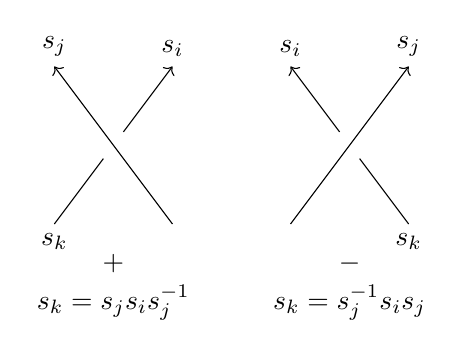
\begin{tikzpicture}
      \draw[->] (0,0) node[below] {$s_k$} -- (1.5, 2) node[above] {$s_i$};
      \fill[white] (0.75, 1) circle (6pt);
      \draw[->] (1.5, 0)--(0, 2) node[above] {$s_j$};
      \node at (0.75, -0.5) {$+$};
      \node at (0.75, -1) {$s_k=s_j s_i s_j^{-1}$};

      \draw[->] (4.5, 0) node[below] {$s_k$} --(3, 2) node[above] {$s_i$};
      \fill[white] (3.75, 1) circle (6pt);
      \draw[->] (3, 0)--(4.5, 2) node[above] {$s_j$};
      \node at (3.75, -0.5) {$-$};
      \node at (3.75, -1) {$s_k=s_j^{-1} s_i s_j$};
    \end{tikzpicture}
  \end{center}
\end{definition}

Take $G=\pi_1(S^3-K)$. Using the Mayer-Vietoris sequence we can show that $G^{ab}=\Z$ regardless of the structure of $K$. Thus we need to work more carefully with $G$ to obtain a reasonable invariant. Consider the following two exact sequences
\begin{center}
  \begin{tikzcd}
    0\arrow[r] & K=[G, G]\arrow[r]\arrow[d] & G\arrow[r]\arrow[d] & \Z \arrow[r]\arrow[d, "id" right] & 0 \\ 
    0 \arrow[r] & K^{ab} \arrow[r] & G^{mab} \arrow[r] & \Z \arrow[r] & 0
  \end{tikzcd}
\end{center}
where both arrows $K\to K^{ab}$ and $G\to G^{mab}$ are quotient maps of $[K, K]$.

\begin{lemma}\label{jadro abeliazniacji}
  Let $s_1,..., s_n$ be the generating set of $G$ and take $a_i=s_is_1^{-1}$ for $i=2,...,n$ and $a_1=s_1$ to be the new generating set. Then $K$ is generated by $s_1^{k}a_is_1^{-k}$ for $k\in\Z$ and $i=2,...,n$.
\end{lemma}

\begin{proof}
  {\large\color{red}TODO}
\end{proof}

Thanks to \cref{jadro abeliazniacji} we can now define the structure of $\Z[\Z]$ module on $K^{ab}$ by
$$t(a_i)=s_1a_is_1^{-1}$$
for $i=2,...,n$. From now on we will think of $K^{ab}$ as a $\Z[\Z]$-module.

\begin{definition}[Alexander matrix]
  Let $G$ be the fundamental group of a knot $K$. Consider the following resolution of $\Z[\Z]$-module $K^{ab}$
  \begin{center}
    \begin{tikzcd}
      ...\arrow[r] & \Z[\Z]^a\arrow[r, "A_D"] & \Z[\Z]^b\arrow[r] & K^{ab}\arrow[r] & 0
    \end{tikzcd}
  \end{center}
  The matrix associated with homomorphism $A_D$ is called the \buff{Alexander matrix} of $G$.
\end{definition}

When $G$ has the Wirtinger presentation with $n$ generators, then $K^{ab}$ has resolution 
\begin{center}
  \begin{tikzcd}
    0\arrow[r] & \Z[\Z] \arrow[r] & \Z[\Z]^{n-1} \arrow[r, "A_D"] & \Z[\Z]^n \arrow[r] & K^{ab} \arrow[r] & 0
  \end{tikzcd}
\end{center}











% \section{Knot coloring}

Let $R$ be any commutative ring with identity, let $M$ be a module with one generator and $\phi:M^3\to M$ be a homomorphism such that for every $m\in M$
%$M$ be any \textbf{\color{red}finitely generated} $R$-module and $\phi:M^3\to M$ be a homomorphism such that for every $m\in M$ 
\begin{equation}\label{phi allows for trivial colorings}
  \phi(m,m,m)=0.
\end{equation}
Notice that if $\phi(u,i,o)=au+bi+co$, then aforementioned equality demands that $(a+b+c)\in \ann(M)$.

Take $K$ to be any knot with diagram $D$ with $s$ arches and $x$ crossings.

\begin{lemma}
  For diagrams of knots other than $0_1$, the number of segments $s$ is equal to the number of crossings $x$.
\end{lemma}

\begin{proof}
  Every crossing has $2$ arcs that go below it and every arc has two bottom ends that are created when this segment disappears below another segment. Thus 
  $$2\cdot \#\text{arches} = \#\text{bottom ends} = 2\cdot \#\text{crossings}.$$
\end{proof}

\begin{definition}\label{coloring definition primitive}
  We say that $C\subseteq M^s$ is a \emph{coloring module} of the diagram $D$ with elements from $M$ if it 
  \begin{enumerate}
    \item {\color{orange}has $s$ generators, each corresponding to one arc of the diagram}, 
    \item and for every $u, i, o\in C$ that correspond to arcs meeting in one crossing, $\phi(u,i,o)=0$.
  \end{enumerate}
  \begin{center}
    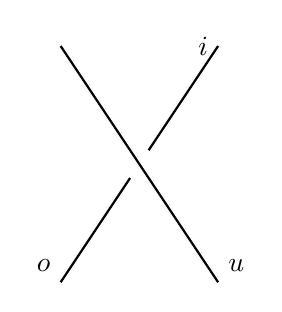
\begin{tikzpicture}
      \draw[thick] (0,0) node[above left] {$o$} --(2, 3) node [left] {$i$};
      \fill[white] (1, 1.5) circle (6pt);
      \draw[thick] (0, 3)--(2, 0) node[above right] {$u$};
    \end{tikzpicture}
  \end{center}
\end{definition}

Notice that condition stated in \cref{phi allows for trivial colorings} makes it possible to color every diagram trivially, that is by assigning the same element of $M$ to every arc of $D$.

Approach to coloring taken in \cref{coloring definition primitive} gives a lot of information about coloring with elements of one specific module $M$ and if one was to change the module to some $M'\neq M$, almost all information gathered for previous coloring would be now ineffectual. Consider the following example.
%it is rather difficult to extrapolate it for other modules. Consider the following example.
%it is rather difficult to use it for other modules. Consider the following example.

\begin{example}
  Take $R=\Z$ with $\phi(x, y, z)=2x-y-z$ and consider the trefoil knot $3_1$. If we take $M=\Z$ then $K$ admits only the trivial coloring module: 
  $$C_M=\{(x, x, x)\;:\;x\in\Z\}.$$ 
  However, if we take $M'=\Z_3$ then there exists a non-trivial coloring like the one presented in \cref{trefoil knot diagram 1}.
  \begin{figure}[h]\centering
    \begin{tikzpicture}[bgnd/.style={circle, fill=white, draw=white}]
       \begin{knot}[
         consider self intersections,
         flip crossing=2,
         clip width=20,
         ]
         \strand[thick]
         (90:3) to[out=180,in=-120,looseness=2]
         (-30:3) to[out=60,in=120,looseness=2]
         (210:3) to[out=-60,in=0,looseness=2] (90:3);
       \end{knot}

       \node[bgnd] at (90:3) {$0$};
       \node[bgnd] at (-30:3) {$1$};
       \node[bgnd] at (210:3) {$2$};
  \end{tikzpicture}
 \caption{The trefoil knot $3_1$ does not allow for nontrivial coloring over $M=\Z$ but it is possible to color it with $M=\Z_3$.\label{trefoil knot diagram 1}}
\end{figure}
\end{example}

Another approach to defining coloring module of a knot diagram $D$ would be by starting with identifying arches with generators $(0,..., 1, ..., 0)$ of $M^s$. Then, we might define a homomorphism
$$f:M^s\to M^x$$
such that arches building one crossing follow rules set by $\phi$.

% We might want to start defining coloring by defining a homomorphism
% $$f:M^s\to M^x$$
% which identifies coordinates with arcs in $D$ and follows $\phi$ on triples of coordinates that build one crossing. 

\begin{definition}\label{coloring definition as kernel}
  Module $\ker f$ is a coloring module of diagram $D$ with elements of $M$.
\end{definition}

Henceforth, we will call $f$ described above a \textbf{coloring homomorphism} for chosen $R$, $M$ and $\phi$.

\begin{corollary}\label{rownowaznosc definicji}
  \Cref{coloring definition primitive} and \cref{coloring definition as kernel} are equivalent for one dimensional modules.
\end{corollary}

\begin{proof}
  {\large\color{red}TO DO}
\end{proof}

Despite the fact that it is the kernel of $f$ that contains colorings, examining the coloring homomorphism itself gives more information about diagram $D$. We might consider $f$ as a $s\times s$ matrix and if $R$ is a PID module, then we can represent this matrix in Smith's normal form. 
%This representation contains information about the kernel over the specific module $M$ and ring $R$ but also shows how to change $M$ and even $R$ to obtain a different coloring.

\begin{proposition}
  Let $A$ be the Smith's normal form of $f$. Columns of $A$ comprised only of zeros and zero divisors contribute to the coloring module. %Moreover, non-unit elements that appear on the diagonal hint at what other colorings are admissible.
\end{proposition}

\begin{proof}
  An immediate result of \cref{rownowaznosc definicji}. The second part 
%  {\large\color{red}TUTAJ WOGÓLE POTRZEBA COKOLWIEK DOWODZIĆ?}
\end{proof}

%Furthermore, if $R$ is a Noetherian ring, then every finitely generated module is a quotient of a free module with the same number of generators. Thus, taking $M$ to be any finitely generated module over $R$ gives us information about coloring with any other module with equal number of generators.

{\color{blue}
If $R$ is a Noetherian ring, then every finitely generated module is a quotient of a free module with the same number of generators. Thus, we might want to take $M$ to be a finitely generated free $R$-module rather than any one dimensional $R$-module. This allows us to send $M$ to any other $R$-module with at most $\dim (M)$ generators to obtain a different coloring.
}

%Usually, it is the irreversible elements from the diagonal of Smith's form $f$ that hint at what colorings are admisible. Consider the following example.

The nonzero elements that appear on the diagonal of the normal form of the coloring homomorphism hint at what colorings over the ring $R$ are admissible. Consider the following example.

\begin{example}\label{ex2}
  As before, take $R=\Z$ and $\phi(x, y, z)=2x-y-z$. Taking $M=\Z$ we have $f:\Z^3\to \Z^3$ for trefoil knot to be a matrix
  $$ 
  \begin{pmatrix}
    2 & -1 & -1 \\ 
    -1 & 2 & -1 \\ 
    -1 & -1 & 2
  \end{pmatrix}
  $$ 
  with Smith's normal form
  $$
  \begin{pmatrix}
    -1 & 0 & 0 \\ 
    0 & 3 & 0\\ 
    0 & 0 & 0
  \end{pmatrix}
  $$
  The normal form of the coloring homomorphism contains a $3$, hinting that $\Z/(3)$ allows for a non-trivial coloring. Send $M=\Z$ to $M'=\Z_3$ by taking all coefficient modulo $3$ to obtain the new Smith's normal form of $f$ to be
  $$
  \begin{pmatrix}
    -1 & 0 & 0 \\ 
    0 & 0 & 0\\ 
    0 & 0 & 0
  \end{pmatrix}
  $$
  which informs about the nontrivial coloring presented in \cref{trefoil knot diagram 1}, that was not allowed over $\Z$.
\end{example}


%
% \section{Coloring oriented diagrams}

In the previous section we defined coloring of a diagram without an orientation. Such a diagram has only one type of crossing, while in a diagram for which an orientation was chosen, two types of crossings are distinguishable in any knot diagram (see \cref{fig two crossings}).

\begin{figure}[h]\centering 
    \begin{tikzpicture}
      \draw[<-, ,thick] (0,0) node[above left] {$o$}--(9/4, 3) node[above left] {$i$};
      \fill[white] (9/8, 1.5) circle (8pt);
      \draw[->, thick] (0, 3)--(9/4, 0) node [above right] {$u$};

      % \node at (-0.1, 0.6) {$u$};
      % \node at (9/4+0.1, 0.6) {$o$};
      % \node at (9/4+0.1, 2.4) {$i$};
      
      \draw[->, thick] (4, 3)--(4+9/4, 0);
      \fill[white] (4+9/8, 1.5) circle (8pt);
      \draw[<-, ,thick] (4,0)--(4+9/4, 3);

      % \node at (-0.1, 0.6) {$u$};
      % \node at (9/4+0.1, 0.6) {$o$};
      % \node at (9/4+0.1, 2.4) {$i$};

      \node at (9/8, -0.6) {$+$};
      \node at (4+9/8, -0.6) {$-$};
    \end{tikzpicture}
    \caption{\label{fig two crossings} Two types of crossings in oriented knot diagram.}
\end{figure}

In the case of a diagram with orientation, we must chose which type of crossing is considered by $\phi$. If not explicitly stated otherwise, we will choose $\phi$ to determine the rules of coloring for crossing of type $+$ as seen in \cref{fig two crossings}. 

If $u$, $i$, $o$ are labels assigned to arches creating a type $+$ crossing that constitute a coloring, then we might write 
$$0=\phi(u, i, o)=au+bi+co.$$
Taking $c$ to be a unit, we get the following equation for the label of the arch leaving the crossing:
$$o=-c^{-1}au-c^{-1}bi.$$

Those assumption allow us to write a $2\times 2$ matrix $A_+$ with terms in $R$ such that multiplying an element $(u, i)\in M^2$ by $A_+$ will return $(o, u)\in M^2$. This means that $A_+:M^2\to M^2$ is the operator taking labels of incoming arches as input and returning labels of segments which leave the crossing.
$$
A_+=\begin{pmatrix}
  -c^{-1}a & -c^{-1}b \\ 
  1 & 0
\end{pmatrix}
$$
It is convenient to take $c=-1$.

Allowing the following Reidemeister's move
\begin{center}
  \begin{tikzpicture}
    \draw[thick, ->] (1, 0) to [out=180+30, in=180-30] (1, -3);
    \fill[white] (0.5, -0.5) circle (6pt);
    \fill[white] (0.5, -2.5) circle (6pt);
    \draw[thick, ->] (0, 0) to [out=-30, in=30] (0, -3);

    \draw[dashed] (0.5, -0.5) circle (10pt);
    \draw[dashed] (0.5, -2.5) circle (10pt);
    \node at (-0.5, -0.5) {$+$};
    \node at (-0.5, -2.5) {$-$};

    \draw[thick, ->] (3, 0) to[out=-70, in=70] (3, -3);
    \draw[thick, ->] (4, 0) to[out=180+70, in=180-70] (4, -3);

    \draw[->, snake it] (1.3, -1.5)--(2.7, -1.5);
  \end{tikzpicture}
\end{center}
gives equality
$$A_-A_+=Id_2,$$
where $A_+$ is the matrix of operator for $+$ type crossing and $-$ - for the $-$ type crossing. Take $\alpha u+\beta i+\gamma o=0$ to be the coloring rule for crossings of type $-$. Once again, for the sake of convenience $\gamma =-1$ and the matrix $A_-$ must be of form
$$
A_-=\begin{pmatrix}
  \beta & \alpha \\ 
  0 & 1 
\end{pmatrix},
$$
meaning that 
$$
\begin{cases}
  b\beta =1\\ 
  b\alpha -a=0.
\end{cases}
$$

Consider another Reidemeister's move
\begin{center}
  \begin{tikzpicture}
    \pic[
braid/.cd,
every strand/.style={thick},
strand 1/.style={red},
strand 2/.style={green},
gap=.2,
height=1.3cm,
width=1.5cm
] {braid={s_2^{-1} s_1^{-1}  s_2^{-1} }};
\draw[thick, red, ->] (0, 0.1)--(0,0);
\draw[thick, green, ->] (1.5, 0.1)--(1.5, 0);
\draw[thick, ->] (3, 0.1)--(3, 0);

  \draw[->, snake it] (3.5, 2)--(4.5, 2);

\begin{scope}[shift={(5, 0)}]
  \pic[
    braid/.cd,
    every strand/.style={thick},
    strand 1/.style={red},
    strand 2/.style={green},
    gap=.2,
    height=1.3cm,
    width=1.5cm
  ] {braid={s_1^{-1} s_2^{-1} s_1^{-1} }};
  \draw[thick, ->] (0, 0.1)--(0,0);
  \draw[thick, ->] (1.5, 0.1)--(1.5, 0);
  \draw[thick, ->] (3, 0.1)--(3, 0);
\end{scope}
  \end{tikzpicture}
\end{center}
Applying $A_\pm$ to each crossing separately yields the following relations
$$
\begin{cases}
  ba = ab \\ 
  a(a+b)=a.
\end{cases}
$$

We must assume that both $b$ and $\beta$ are units. In the most general situation, we are considering coloring modules as modules over the ring
$$R=\Z[s, t, t^{-1}]/\{s^2+st-s\},$$
with $a$ being send to $s$ and $b$ being send to $t$. However, it can be beneficial to at first assume yet another relation: 
$$a+b=1,$$
meaning that we are considering coloring as $\Z[t, t^{-1}]$ module.

Coloring a knot with $\Z[t, t^{-1}]$ module allows us to obtain information about coloring over $\Z$ or many other commutative rings by sending $t$ to a unit in the ring in question.

\begin{example}\label{ex3}
  Consider knot $4_1$ with diagram $D$ as seen in \cref{fig:4_1:coloring} and ring $R=\Z[t, t^{-1}]$. Take function $\phi:M^3\to M$ to be defined as
  $$\phi(u, i, o)=(1-t)u+ti-o$$

  The coloring homomorphism $f$ is then defined by the matrix
  $$
  f=\begin{pmatrix}
    1-t & t & -1 & 0 \\
    t^{-1} & -1 & 0 & 1-t^{-1}\\
    0 & 1-t^{-1} & t^{-1} & -1\\
    -1 & 0 & 1-t & t
  \end{pmatrix}
  $$
  Changing the coefficients in $R$ to $\Q$ yields the following Smith's normal form for $f$:
  $$
  S=\begin{pmatrix}
    -1 & 0 & 0 & 0 \\
    0 & -1 & 0 & 0\\
    0 & 0 & t^2-3t+1 & 0\\
    0 & 0 & 0 & 0\\
  \end{pmatrix}
  $$
  Notice, that $\det S=t^2-3t+1$, which is the Alexander polynomial of $4_1$.

  \begin{figure}[h]\centering
    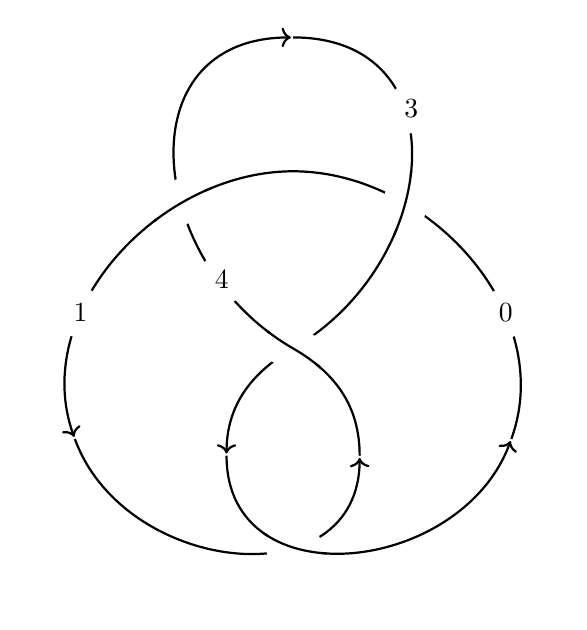
\begin{tikzpicture}[bgnd/.style={circle, fill=white, draw=white}]
      %\node[opacity=0.2] at (0,0) {\includegraphics[width=0.5\textwidth]{./rozdzialy/4_1-3d.png}};
      \coordinate (a1) at (90: 3.5);
      \coordinate (a2) at (-30:3.2);
      \coordinate (a3) at (210: 3.2);
      \coordinate (a4) at (0,-0.45);
      \coordinate (a5) at (-65:2);
      \coordinate (a6) at (180+65: 2);
      \coordinate (a7) at (90: 1.8);

      %\foreach \i in {1, ..., 7} \fill (a\i) circle (2pt);
      \begin{knot}[
        %consider self intersections,
        flip crossing=2,
        clip width=20,
        ]
        \strand[thick, ->]
        (a1) to [out=0, in=30, looseness=1.4]
        (a4) to [out=210, in=90, looseness=1] (a6);
        \strand[thick, ->]
        (a6) to [out=-90, in=250, looseness=1.3] (a2);
        \strand[thick, ->] (a2) to[out=70, in=0] (a7) to[out=180, in=110] (a3);
        \strand[thick, ->] (a3) to[out=290, in=-90, looseness=1.3] (a5);
        \strand[thick, ->] (a5) to[out=90, in=-30, looseness=1] (a4) to [out=150, in=180, looseness=1.4] (a1);
      \end{knot}

      \node[bgnd] at (60:3) {$3$};
      \node[bgnd] at (0:2.7) {$0$};
      \node[bgnd] at (-180:2.7) {$1$};
      \node[bgnd] at (155:1) {$4$};
    \end{tikzpicture}
    \caption{\label{fig:4_1:coloring} Coloring of knot $4_1$ with elements from $\Z_5$.}
  \end{figure}

  Now, consider a homomorphism $\Z[t, t^{-1}]\to \Z$ defined by $t\mapsto -1$. This yields a new matrix for $f$, with Smith's normal form:
  $$f=\begin{pmatrix}
    -1 & 0 & 0 & 0\\
    0 & 1 & 0 & 0\\
    0 & 0 & 5 & 0\\
    0 & 0 & 0 & 0
  \end{pmatrix}$$
  The matrix above hints at existence of a coloring with elements from $\Z_5$, one of which is presented in \cref{fig:4_1:coloring}.
\end{example}

%
% \section{Reducing normal form of a matrix}

In \cref{coloring definition as kernel} we defined the coloring module of a diagram $D$ as the kernel of coloring homomorphism. We might also want to extend this homomorphism to a short exact sequence
\begin{center}
  \begin{tikzcd}
    0\arrow[r] & \ker f\arrow[r, hookrightarrow] & M^s\arrow[r, "f"] & M^s\arrow[r, two heads] & \coker f \arrow[r] & 0
  \end{tikzcd}
\end{center}
and ask what information can be obtained from studying $\coker f$.

In \cref{ex2,,ex3} nontrivial coloring was admissible only in modules $M/\mathfrak{a}$, where $\mathfrak{a}$ is the ideal spanned by a portion of terms that appear on the diagonal of Smith's normal form of $f$. In the same examples, we observe also that $\coker f=R^k\oplus R/\mathfrak{a}$. For the knot $3_1$ it was $\coker f=\Z\oplus \Z_3$, while in the case of knot $4_1$ $\coker f=\Z\oplus \Z_5$.

\begin{proposition}
  Let $f$ be a coloring homomorphism of an oriented diagram $D$. If $\coker f=R/\mathfrak{a}_1\oplus...\oplus R/\mathfrak{a}_k$ then $D$ can be colored with elements from $R/\mathfrak{a}_i$ for $i=1,..., k$.
\end{proposition}

\begin{proof}
  {\color{red}To się powinno sprowadzić do rozwiązywania układu równań przy pomocy macierzy}.
\end{proof}

The coloring homomorphism $f$ of a diagram $D$ carries a lot of information about the knot whose diagram it is. However, $f$ in itself is not a knot invariant. The dimensions of its matrix will change if a new crossing is created, see the following example.

\begin{example}\label{ex4}
  We take knot $3_1$ with additional crossing, $R=\Z[t, t^{-1}]$ and $M=\Z[t, t^{-1}]$ with $\phi$ as in \cref{ex3}. The coloring homomorphism has matrix
  $$
  \begin{pmatrix}
    1-t & t & -1 & 0 \\ 
    t & -1 & 0 & 1-t \\ 
    -1 & 1-t & 0 & t \\ 
    0 & 0 & 1 & -1 
  \end{pmatrix}
  $$
  with normal form
  $$
  \begin{pmatrix}
    -1 & 0 & 0 & 0\\ 
    0 & 1 & 0 & 0 \\ 
    0 & 0 & -t^2+t-1 & 0 \\ 
    0 & 0 & 0 & 0 &
  \end{pmatrix}
  $$
  which after evaluation at $t=-1$ yields
  $$
  \begin{pmatrix}
    -1 & 0 & 0 & 0\\ 
    0 & 1 & 0 & 0 \\ 
    0 & 0 & -3 & 0 \\ 
    0 & 0 & 0 & 0 &
  \end{pmatrix}
  $$
  which differs from matrix obtained in \cref{ex2} by just one trivial.
  \begin{figure}[h]\centering 
    \begin{tikzpicture}
    \begin{knot}[
      clip width=40,
      consider self intersections,
      ignore endpoint intersections=false, 
      flip crossing=2
      ]
      \strand[thick, ->] 
        (90:3) to [out=180, in=-90-30, looseness=2] 
        (-30:3);
      \strand[thick, ->] (-30:3) to [out=60, in=90, looseness=1.5] 
        (200:3.5); 
      \strand[thick, ->] (200:3.5) to[out=-90, in=-30, looseness=1.5] 
        (210:5);
      \strand[thick, ->] (210:5) to[out=180-30, in=180-30, looseness=1.5] 
        (210:3); 
      \strand[thick, ->] (210:3) to[out=-30, in=0, looseness=2]
        (90:3);
    \end{knot}
    \end{tikzpicture}
    \caption{Diagram of knot $3_1$ with additional crossing.\label{trefoil z dodatkowym skrzyzowaniem}}
  \end{figure}
\end{example}

The nontrivial term on the diagonal in \cref{ex4} is the same as in \cref{ex2}. The difference between matrices obtained in those two examples are their dimensions.

\begin{definition}\label{equivalence of matrices definition}
  % Let $f$ be a coloring homomorphism of diagram $D$ with Smith's normal form 
  % $$
  % S=\begin{pmatrix}
  %   a_1 & 0 & 0 & \hdots & 0 & \hdots & 0 \\ 
  %   0 & a_2 & 0\\ 
  %   0 & 0  & \ddots & & \vdots & & \vdots \\ 
  %       & & & a_k \\ 
  %     0 & &\hdots &  & 0 & \hdots & 0 \\ 
  %     \vdots & & & & \vdots & & \vdots\\ 
  %     0 & & \hdots & & 0 & \hdots & 0
  %   \end{pmatrix}
  % $$
  % We will define 
  %
  %
  Let $A$, $B$ be matrices with entries from a PID ring $R$. We will say that they are equivalent ($A\sim B$) if and only if their Smith's normal form has the same nonzero and nonunit terms.
\end{definition}

\begin{example}
  Matrices of coloring homomorphisms over the ring $\Z$ of knot $3_1$ presented in \cref{ex2,,ex4} are both equivalent to a $1\times 1$ matrix $\begin{pmatrix}3\end{pmatrix}$.
\end{example}

\begin{theorem}
  Equivalence class of matrices under relation $\sim$ defined in \cref{equivalence of matrices definition} is a knot invariant.
\end{theorem}







\bigskip

\rule{\textwidth}{1pt}
\bigskip

\begin{example} 
  First, consider the knot $6_1$ with diagram as seen in \cref{fig:6_1:knot}, ring $R=\Z[t, t^{-1}]$ and $M=R$. We calculate that
\begin{figure}[h]\centering
  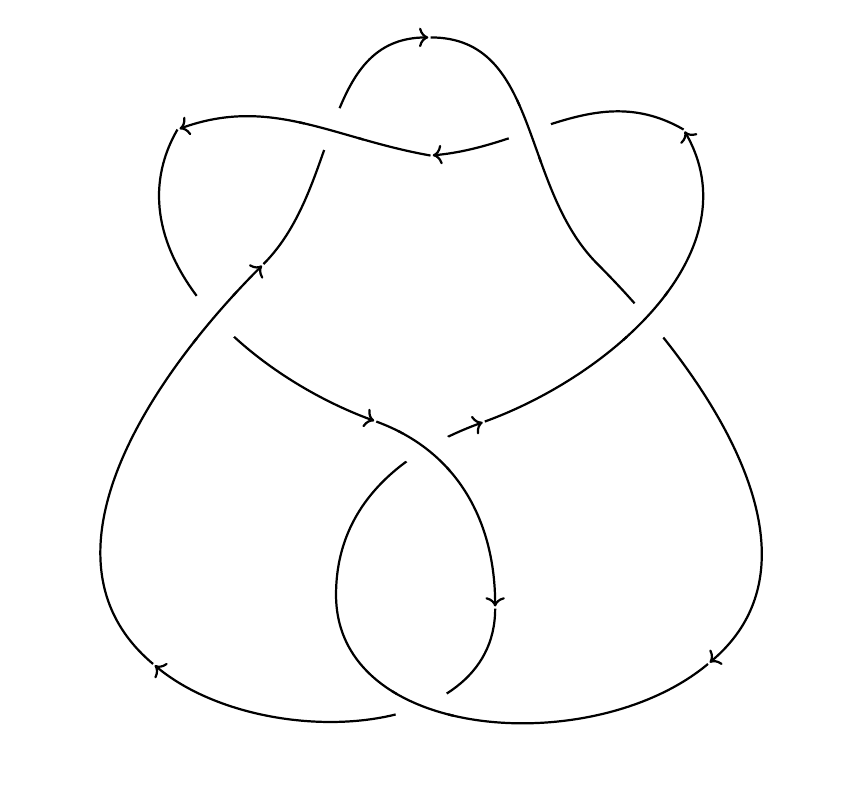
\begin{tikzpicture}[bgnd/.style={circle, fill=white, draw=white}]
    %\node[opacity=0.2] at (0,0) {\includegraphics[width=0.7\textwidth]{./rozdzialy/6_1-3d.png}};

    \coordinate (a0) at (0,0);
    \coordinate (a1) at (90:5);
    \coordinate (a2) at (45:3);
    \coordinate (a3) at (-40:4.6);
    \coordinate (a4) at (-120:2.4);
    \coordinate (a5) at (10:0.7);
    \coordinate (a6) at (50:5);
    \coordinate (a7) at (90:3.5);
    \coordinate (a8) at (180-50:5);
    \coordinate (a9) at (170:0.7);
    \coordinate (a10) at (-70:2.4);
    \coordinate (a11) at (220:4.6);
    \coordinate (a12) at (180-45:3);

    %\foreach \i in {0,...,12} \fill (a\i) circle (2pt);

    \begin{knot}[
      clip width=20, 
      flip crossing=1,
      flip crossing=3,
      flip crossing=6
      ]
      \strand[thick, ->] (a1) to[out=0, in=90+45] (a2) to[out=-45, in=40] (a3);
      \strand[thick, ->] (a3) to[out=220, in=-90] (a4) to[out=90, in=200] (a5);
      \strand[thick, ->] (a5) to[out=20, in=-60] (a6);
      \strand[thick, ->] (a6) to[out=150, in=5] (a7);
      \strand[thick, ->] (a7) to[out=170, in=20] (a8);
      \strand[thick, ->] (a8) to[out=240, in=160] (a9);
      \strand[thick, ->] (a9) to[out=-20, in=90] (a10);
      \strand[thick, ->] (a10) to[out=-90, in=-40] (a11);
      \strand[thick, ->] (a11) to[out=140, in=180+45] (a12);
      \strand[thick, ->] (a12) to[out=45, in=180] (a1);
    \end{knot}

    %\node at (80: 5) {$A$};
    %\node at (-40:4) {$B$};
    %\node at (45:5.5) {$C$};
    %\node at (135:5.5) {$D$};
    %\node at (-1.5,0.1) {$E$};
    %\node at (220:4) {$F$};
    %
    %\node[bgnd] at (70:4.7) {$1$};
    %\node[bgnd] at (25:3.9) {$2$};
    %\node[bgnd] at (-90:3) {$3$};
    %\node[bgnd] at (90:0.5) {$4$};
    %\node[bgnd] at (110:4.7) {$5$};
    %\node[bgnd] at (180-25:3.9) {$6$};

    %\draw[dashed] (70: 4) circle (0.4);
    %\draw[dashed] (28: 3.1) circle (0.4);
    %\draw[dashed] (-90:3.5) circle (0.4);
    %\draw[dashed] (-90:0.15) circle (0.4);
    %\draw[dashed] (180-28:3.1) circle (0.4);
    %\draw[dashed] (110:4) circle (0.4);
  \end{tikzpicture}
  \caption{\label{fig:6_1:knot}Diagram of knot $6_1$.}
\end{figure}
$$f=\begin{pmatrix}
  -1 & 0 & 0 & 0 & 0 & 0 \\ 
  0 & -1 & 0 & 0 & 0 & 0 \\ 
  0 & 0 & t & 0 & 0 & 0 \\ 
  0 & 0 & 0 & t & 0 & 0 \\ 
  0 & 0 & 0 & 0 & -2t^{-2}+5t^{-1}-2 & 0 \\ 
  0 & 0 & 0 & 0 & 0 & 0 
\end{pmatrix}$$
which agrees with the Alexander polynomial of $6_1$. Now, the reduced form of $f$ would be 
$$
\begin{pmatrix}
  -2t^{-2}+5t^{-1}-2
\end{pmatrix}
$$
a $1\times 1$ matrix.

There is another knot with Alexander polynomial equal $-2t^{-2}+5t^{-1}-2$: $9_{46}$. Using diagram in \cref{fig:9_46:knot} it can be calculated that  
\begin{figure}[h]\centering
  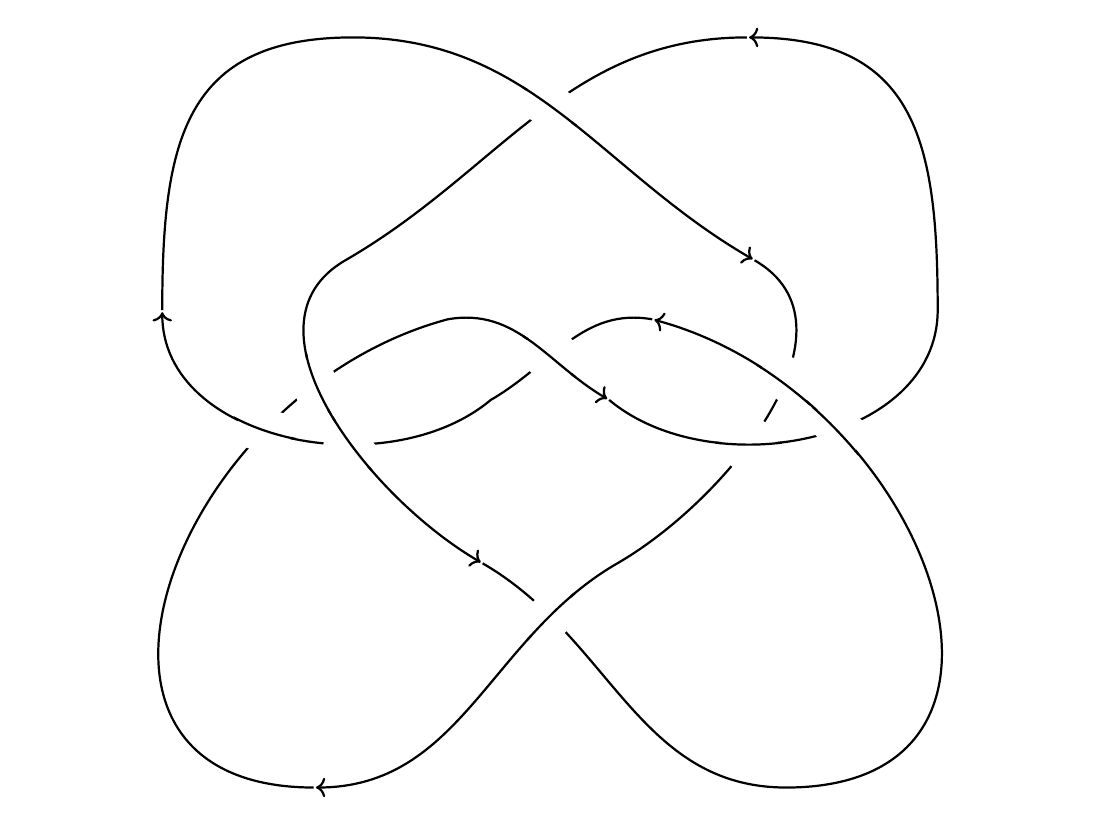
\begin{tikzpicture}[bgnd/.style={circle, fill=white, draw=white}]
    %\node[opacity=0.2] at (0,0) {\includegraphics[width=0.7\textwidth]{./rozdzialy/6_1-3d.png}};

    \coordinate (a0) at (0,0);
    \coordinate (a1) at (60:5);
    \coordinate (a2) at (150:3);
    \coordinate (a3) at (-110:2.5);
    \coordinate (a4) at (-60:6);
    \coordinate (a5) at (30:1.5);
    \coordinate (a6) at (200:0.8);
    \coordinate (a7) at (170:5);
    \coordinate (a8) at (120:5);
    \coordinate (a9) at (30:3);
    \coordinate (a10) at (-70:2.5);
    \coordinate (a11) at (180+60:6);
    \coordinate (a12) at (150:1.5);
    \coordinate (a13) at (-20:0.8);
    \coordinate (a14) at (10:5);

    %\foreach \i in {0,...,14} \fill (a\i) circle (2pt);

    \begin{knot}[
      clip width=20, 
      consider self intersections,
      ignore endpoint intersections=false,
      %draft mode=crossings,
      flip crossing=1,
      flip crossing=4,
      flip crossing=7, 
      flip crossing=9
      ]
      \strand[thick, ->] 
        (a1) to [out=180, in=30]
        (a2) to [out=210, in=150]
        (a3);
      \strand[thick, ->]
        (a3) to [out=-30, in=180] 
        (a4) to [out=0, in=-15, looseness=1.5] 
        (a5);
      \strand[thick, ->]
        (a5) to [out=170, in=30] 
        (a6) to [out=220, in=-90] 
        (a7);
      \strand[thick, ->]
        (a7) to [out=90, in=180, looseness=1.3] 
        (a8) to [out=0, in=150] 
        (a9);
      \strand[thick, ->]
        (a9) to [out=-30, in=30]
        (a10) to [out=210, in=0] 
        (a11);
      \strand[thick, ->]
        (a11) to [out=180, in=180+15, looseness=1.5] 
        (a12) to [out=10, in=150]
        (a13);
      \strand[thick, ->]
        (a13) to [out=-40, in=-90]
        (a14) to [out=90, in=0, looseness=1.3]
        (a1);
      \fill[yellow] (-10:3.7) circle (6pt);
    \end{knot}
  \end{tikzpicture}
  \caption{\label{fig:9_46:knot}Diagram of knot $9_{46}$.}
\end{figure}
$$f=\begin{pmatrix}
  1 & 0 & 0 & 0 & 0 & 0 & 0 & 0 & 0 \\ 
  0 & t^{-1} & 0 & 0 & 0 & 0 & 0 & 0 & 0 \\ 
  0 & 0 & t^{-1} & 0 & 0 & 0 & 0 & 0 & 0\\ 
  0 & 0 & 0 & t  & 0 & 0 & 0 & 0 & 0 \\ 
  0 & 0 & 0 & 0 & t  & 0 & 0 & 0 & 0 \\ 
  0 & 0 & 0 & 0 & 0 & t  & 0 & 0 & 0\\ 
  0 & 0 & 0 & 0 & 0 & 0 & 2t-t^2 & 0 & 0 \\ 
  0 & 0 & 0 & 0 & 0 & 0 & 0 & t^{-2}-2t^{-1} & 0\\ 
  0 & 0 & 0 & 0 & 0 & 0 & 0 & 0 & 0
\end{pmatrix}$$
where 
$$\det f= (2t-t^2)(t^{-2}-2t^{-1})=2t^{-1}-5+2t$$
is also the Alexander polynomial. The reduced form of $f$ is
$$
\begin{pmatrix}
  2t-t^2 & 0 \\ 
  0      & t^{-2}-2t^{-1}
\end{pmatrix}
$$
which is significantly different than the one for $6_1$.
\end{example}

{\large\color{red}TO DO: sprawdzić te węzły wyżej za pomocą pow. Seiferta, czy mają różne moduły Alexandera}


\bibliographystyle{plain}
\bibliography{literatura}
%
\end{document}
